\documentclass[10pt]{article}
% MAXIMUM VIEWER COMPATIBILITY. pdfTeX writes PDF 1.5 by default, which uses a
% compressed cross reference stream and object streams. Both are legal and both
% are what GitHub's in browser viewer most often fails to render, reporting the
% file as invalid when it is not. Dropping to 1.4 with object compression off
% writes a classic xref table, which every viewer reads. It costs some file size
% and nothing else.
\pdfminorversion=4
\pdfobjcompresslevel=0
\pdfcompresslevel=9

\usepackage[margin=1in]{geometry}
\usepackage{amsmath,amssymb}
\usepackage{booktabs}
\usepackage{graphicx}
\usepackage{array}
\usepackage[hidelinks]{hyperref}
\usepackage{xcolor}
% Everything revised in this draft is marked in red: the move to two periods and
% the responses to the comments on the previous version. The change of
% terminology from "the disorder" to "a SUD" runs through the whole note and is
% NOT marked, since colouring every instance would colour half the document.
% fill.py wraps in  every number that MOVED against numbers_prev.json, so
% the note marks a changed number automatically rather than by hand. Set it to red
% so a recalibration shows up as red without anyone having to find the numbers.
% To clear the marks, copy the current numbers over numbers_prev.json and refill.
%  is the mark fill.py puts on every number that moved since
% numbers_prev.json. It prints as ordinary text: the reader asked not to see the
% pipeline's own bookkeeping in red. The mark survives in the generated .tex,
% so grepping the generated file for the macro finds what moved, and grepping
% .src.tex for the at signs finds every number the stylized pipeline still
% supplies and the quantitative model has yet to replace.
% \textcolor is NOT \long: a red span that crossed a blank line died with
% "Paragraph ended before \@textcolor was complete", and pdflatex then
% returned nonzero, which set -e turned into a build that stopped before
% every checker in build.sh. \color is a switch and survives \par.
% \new MUST RENDER RED. strip_red.py rewrites this line to a passthrough,
% \newcommand{\new}[1]{#1}, so that any \new left after a strip is inert.
% That passthrough was committed once and every \new written afterwards
% went in as plain black text: several rounds of marked edits were
% invisible to the reader, in the intro, the calibration entries and the
% citations alike, while table cells kept showing red because they use
% \textcolor directly. check_red.py now fails the build if this line is
% a passthrough while any \new remains in the file.
\newcommand{\new}[1]{{\color{red}#1}}
% A number not computed yet: a slot to fill, never a guess.
\newcommand{\blank}{\underline{\hspace{2.2em}}}
% A STANDING FLAG, which survives the strip between rounds. \new and \cut both
% mark what changed since the last version and are cleared when the next round
% starts, so neither can carry an open question forward. \query holds one: a
% short red note in the margin asking whether a passage should be there at all.
% It is not prose and must be gone before the note is circulated.
% A FLAG IS A FOOTNOTE, NOT A MARGIN NOTE, AND THAT IS NOT A STYLE CHOICE.
% As a \marginpar it broke float placement: the run reported "Float(s) lost",
% the standard parameters table was never placed, its \label went with it, and
% the three references to it printed as ??. That is the same ?? flagged in the
% margin two rounds ago and explained away then as a stale build; it was this.
% Rebuilt with \query made a no-op the run is clean, which is what identifies
% the cause. Blue, so a flag is never mistaken for a round's red.
\newcommand{\query}[1]{\footnote{\textcolor{blue}{#1}}}
% THE PARAMETER COUNTS AS MACROS, so the two table files can quote them too.
% fill.py only rewrites its placeholders in this file, and the tables are
% \input from
% their own .tex, so a caption saying how many rows its table has could not be
% generated any other way. Counted off the Set column of the tables themselves.
\newcommand{\nmain}{\new{twenty nine}}
\newcommand{\nstd}{twenty six}
% The cut macro below marks a PROPOSED DELETION: red and struck through, so the reader sees what
% would go before it goes. ulem is not in this installation, and a single rule over a
% whole phrase cannot break across lines, so the rule is drawn word by word: each word
% is its own box and TeX breaks between them as usual. The scanner below splits the
% argument on spaces, which is why a cut must not contain a braced group with a space
% inside it. Maths is fine, $14.2$ is one word.
\makeatletter
\newlength{\cw@len}
\newcommand{\cw}[1]{{\settowidth{\cw@len}{#1}%
  \rlap{\textcolor{red}{\rule[0.55ex]{\cw@len}{0.4pt}}}\textcolor{red}{\hspace{0pt}#1}}}
\newcommand{\cut}[1]{\cut@scan#1 \@nil}
\def\cut@scan#1 #2\@nil{\cw{#1}\ifx\relax#2\relax\else\space\cut@scan#2\@nil\fi}
\makeatother
\usepackage[official]{eurosym}
\usepackage{longtable}
\usepackage{titlesec}

\setlength{\parskip}{0.18em}
\newcolumntype{L}[1]{>{\raggedright\arraybackslash}p{#1}}

\renewcommand{\topfraction}{0.92}
\renewcommand{\bottomfraction}{0.85}
\renewcommand{\textfraction}{0.06}
\renewcommand{\floatpagefraction}{0.80}
\setlength{\textfloatsep}{12pt plus 2pt minus 3pt}
\setlength{\intextsep}{10pt plus 2pt minus 3pt}

\newcommand{\notes}[2]{\par\vspace{0.4em}%
  \begin{minipage}{#1}\footnotesize #2\end{minipage}}
% A table's note should start and end exactly where the rules of the table do.
% \tabnote measures the table into a box first and sets the note to that width.
% Captions sit above the tables, and the default gap below one is small enough
% that the title touches the top rule. Set once so every table gets the same air.
\setlength{\belowcaptionskip}{0.6em}
\newsavebox{\ntbox}
\newcommand{\tabnote}[1]{\notes{\wd\ntbox}{#1}}
\titlespacing*{\subsection}{0pt}{1.4em plus 0.3em}{0.7em plus 0.15em}
\titlespacing*{\subsubsection}{0pt}{1.1em plus 0.25em}{0.6em plus 0.15em}

\begin{document}

\begin{center}
\renewcommand{\thefootnote}{\fnsymbol{footnote}}
{\Large\bfseries Children First, Housing Later}\footnote{I thank Ay\c{s}e \.{I}mroho\u{g}lu, Kai Zhao, Joseph Steinberg, Efraim Benmelech, Jonathan Alschech, Ryan Quandt, Christopher Sharp and the seminar participants at the University of Toronto for their helpful comments. The data and replication code are available on GitHub at \url{https://github.com/srotberg/housing_first_children_later}.}\\[0.6em]
{\large Shahar Rotberg}\footnote{Canada Mortgage and Housing Corporation (CMHC). Contact: \url{shahar.rotberg@gmail.com}. Website: \url{www.shaharrotberg.com}. This work was conducted on personal equipment and time. The code used to solve the model is the author's own. The opinions expressed herein do not necessarily represent the views of CMHC.}\\[0.35em]
\today
\end{center}
\renewcommand{\thefootnote}{\arabic{footnote}}
\setcounter{footnote}{0}

\vspace{0.4em}
\begin{center}
\begin{minipage}{0.86\textwidth}
\begin{center}\textbf{Abstract}\end{center}
\noindent Should housing assistance require sobriety? Without externalities, no:
conditionality removes an option from forward-looking households. While
conditionality reduces the externalities drug use imposes on users' children, it also
raises homelessness, an externality that harms children and everyone nearby. A
general-equilibrium model of homelessness, drug use, drug prices and mortality,
calibrated to United States data, captures both externalities, with altruism
matching how much less parents use drugs than non-parents. Full altruism sharply cuts
drug use and homelessness. Conditioning assistance raises homelessness but
substantially cuts drug use, raising welfare in transition and the long run
through children's greater resources and future earnings.

\vspace{0.6em}
\noindent\textit{Keywords:} homelessness; housing vouchers; substance
use disorder; intergenerational transmission; externalities; distortions.

\vspace{0.2em}
\noindent\textit{JEL classification:} I18; I38; H23; R21; J62.
\end{minipage}
\end{center}

\vspace{0.8em}


%======================================================================
\section{Introduction}\label{sec:intro}


On a single night in January 2024 the point-in-time (PiT) count run by the Department
of Housing and Urban Development (HUD) found $771{,}480$ people homeless in the United
States, the most since the count began. In July 2025 an executive order moved the
federal government decisively to one side of a long argument about what to do about
it: it required sobriety in federally funded housing and homelessness programmes.\footnote{Executive Order, \emph{Ending Crime and Disorder on America's
Streets}, 24 July 2025. Reported in
\url{https://www.npr.org/2025/07/24/nx-s1-5479139/trump-homelessness-executive-order-civil-commitment-camping}.} The money followed, redirecting about a third of what the programmes at the time
carried between them away from Housing First and towards programmes conditional on
sobriety.\footnote{See
\url{https://www.npr.org/2025/11/14/nx-s1-5553561/homelessness-housing-funding-trump-administration-hud}.} Whether housing assistance should be conditioned on sobriety is no longer
an academic question. It is policy that decides the welfare of hundreds of
thousands of people.



The argument between the Housing First and Treatment First camps is
usually framed as a contest between two behavioural claims.\footnote{For the case
against Housing First as the federal government now makes it, see the executive order
cited above; for the case for it, see the National Alliance to End Homelessness,
\url{https://endhomelessness.org/blog/ceo-corner-week-of-july-28/}.} Critics of
Housing First say that unconditional assistance is moral hazard: guaranteeing housing
whatever a household does weakens the incentive to stay sober and attached to the
labour market, so use and substance use disorder (SUD) rise, which feeds back to
homelessness, because a SUD costs jobs and a lost job means not only more use but
less ability to pay rent. Critics of Treatment First say that conditionality delays
stable housing for exactly the households least able to wait, worsens their
employment, and makes SUD recovery harder, because the street and shelters are poor places to recover. That too runs in a circle: worse recovery means more disorder, and more
disorder means more homelessness. Both claims have merit, and the
experimental literature has not settled between them, because the trials that could are short.



Randomised trials of Housing First find
large and persistent gains in housing stability and mixed to null effects on substance
use (Tsemberis et al., 2004; Aubry et al., 2016, among others), but they focus on the drug users themselves, and run six to twenty four months, so they cannot
speak to long-run behaviour or to the budget required to fund either policy at
scale. A model can follow what a trial cannot. It can trace the impact of a
policy well beyond the households in the study group, to their children and to others in the economy, and well beyond the length of a trial.

This paper starts from the observation that the debate as framed is
missing the mark, because the moral hazard both sides argue about has nothing
to do with efficiency at all. Consider households that are forward-looking, as in Becker and
Murphy (1988), and that have no self-control problems of the kind modelled with
hyperbolic discounting at the moment they decide whether to start using. Suppose
they account for the true hazard of acquiring a SUD when
they make that decision, as the evidence suggests (Lundborg and Lindgren, 2002; van Ours, 1995; Grossman
and Chaloupka, 1998; Saffer and Chaloupka, 1999; Caulkins, 2001; Gallet, 2014;
Greenwood et al., 2025). Then at the same generosity and the same cost, Housing First
weakly dominates Treatment First for every household. Conditionality removes an
option from an optimiser and gives nothing back.

The case for Treatment First therefore has to rest on something outside the
household's own objective, and this paper focuses on four externalities, which randomised
trials cannot resolve: two that Housing First leaves in place and two that Treatment
First creates.

The two Housing First leaves in place are harms drug use does to the user's
children. The first runs through the household's budget, the \emph{budget
externality}: children live with their parents and share their consumption and their
dwelling, but not the drug, so every unit a parent spends on drugs, and every job a SUD
costs it, is consumption and housing the child goes without. When Treatment First
reduces drug use, it diverts more resources towards children. The second runs through
earnings in adulthood, the \emph{earnings externality}: a child whose parent had a
SUD during its upbringing starts adult life with lower productivity and earns less for
the rest of its life. When Treatment First reduces the SUD, it raises the
earnings of children in adulthood.

The two Treatment First creates both run through homelessness. By denying housing
assistance to drug users, Treatment First exposes more of them to homelessness.
The first externality this creates falls on everyone, the \emph{aggregate
homelessness externality}: every household's utility falls with the share of the
population that is homeless, capturing in a reduced-form way the idea that it is
less safe and pleasant to live in a place with more homelessness, and homeless
households do not internalise the cost their own homelessness imposes on everyone
else. The second externality falls on drug users' children, the \emph{childhood
homelessness externality}: a child lives wherever its parent lives, so a parent put
in a shelter takes the child into the shelter too.

A parent takes the budget, earnings and childhood homelessness externalities into
account only through its altruism, and only in part. How much weight it puts on its
child is calibrated to the difference in drug use between parents and adults
without children in the data. In the 2024 National Survey on Drug Use and Health
(NSDUH), adults without children use drugs
$18.3$ percent more than parents with the same characteristics, so the
weight is set so that removing a parent's concern for its child would raise drug use
in the model by that much. The part of the child's loss a parent does internalise is
thus pinned down by observed behaviour.

Given the degree of altruism, the size of each externality is set by data. The
budget externality depends on how much a user household spends on the drug.
The weight given to drugs in the utility function is set to match the share of their
income that drug users spend on drugs, $16.2$ percent, from retail drug spending
(Midgette et al., 2019) and the incomes of adults who use in the 2024 NSDUH. The
earnings penalty is set from a direct estimate: children exposed in utero to a
Swedish alcohol experiment earn about $24$ percent less as adults
(Nilsson, 2017). The intergenerational transmission of SUD is then left untargeted:
in the model a child of a parent with a SUD is $1.51$ times as likely to
acquire one itself, against $1.5$ to $2.5$ in the data (Mellentin et al., 2016; Yoon
et al., 2013). The childhood homelessness externality carries no earnings penalty at
all. The link between a parent's homelessness and the child's comes from
intergenerational transmission alone, and the model is calibrated to estimates of
earnings transmission from the literature (Solon, 1992; Mazumder, 2005; Chetty et
al., 2014): a child's productivity is correlated with its parent's, and
lower-productivity households are poorer and more likely to be homeless, so their
children are more likely to draw a lower productivity, be poor, and end up
homeless as well. With this mechanism in place, a child of a homeless parent is
$4.92$ times as likely to be homeless itself, against $1.8$ to $2.4$ in the
data (Bassuk et al., 1997). The aggregate homelessness externality is priced as a
disamenity in flow utility, in proportion to the homelessness rate, set from the
contingent valuation in Loubi\`ere et al.\ (2020), where the Europeans willing to pay
anything to end homelessness would pay $0.2$ percent of average annual
earnings a year.

Who bears these externalities depends on who uses drugs, and one mechanism of the
model decides it. Two facts about drug use have to be reproduced together, and the
literature has so far explained them only by assuming that lower-education
households, whose income is lower because of their education, have a stronger
preference for drugs (Greenwood et al., 2025). Drug use is concentrated at the
bottom of the income distribution, where the average user's income is about
$74$ percent of the average in the 2024 NSDUH, and it
is not universal: most households do not use at all, so there is a margin at zero,
with a participation rate of $8.90$ percent among adults aged $26$ and over in the
same survey. To generate both I model drugs as a luxury good bought at a price, which
puts most households at a corner where they optimally consume none. Left to its own
devices, however, that same assumption concentrates use at the \emph{top}, since the
share of income spent on a luxury good rises with income. What reverses the income
gradient, as I show, is the increased mortality risk that comes with a SUD: acquiring
a disorder truncates the expected continuation value of life, and that loss rises
faster than income does, so in equilibrium use concentrates at the bottom.

I proceed with two models, a stylized model for the intuition and a full quantitative
model for the policy analysis. The stylized model is a life-cycle model with three
periods of life (childhood, adulthood and old age) and rational forward-looking
households, who care about consumption, housing and drugs. It shows four things
at their clearest: how and why the income gradient in drug use reverses, how the
value of life and moral hazard pull drug use in opposite directions, how one can find
the optimal degree of homelessness, drug use and SUD, and why the externalities
Treatment First removes outweigh the ones it creates.

In the stylized model, an adult draws a productivity and an unemployment shock, and
chooses how much of the drug to buy; drug users risk acquiring a SUD, and a SUD raises
the chance of dying before old age, the chance of losing employment, and
a job lost to the disorder is not covered by unemployment insurance. It
chooses whether to live in a shelter or in a rental, and it may hold a
means-tested voucher, which is rationed; food assistance puts a floor under its
consumption, so that all households have a positive value of life, which means they have
something valuable to lose by dying. Children live with their parents during the
parents' adulthood and share their resources (except the drugs), and the weight
a parent puts on its child is calibrated, as in the full model, to match the gap in
drug use between parents and adults without children. The aggregate homelessness
externality is in the model too, calibrated \new{to the same willingness to pay} as in the full model. At the end of the
parents' adulthood, their child becomes an adult, and its productivity draw is
penalised if the parent acquired a SUD while the child lived with them. There is no
government budget in the stylized model, so revoked vouchers are not offset by a
higher probability of drawing a voucher for sober households; that is deliberate, so
the mechanisms can be seen clearly, and the quantitative model takes up the detail.
The model is calibrated to United States data.

Welfare is measured using the ex-ante expected utility of newborns,
childhood included, in consumption-equivalent terms, against the world with
rationed Housing First.

This stylized model shows starkly how the income gradient reverses. It separates the
two penalties a disorder carries (death and unemployment). Scaled from nothing to
$2$ times its calibrated value, with the other penalty switched off, the death penalty takes the average user
from $3.54$ times average income to $0.52$ times it; the unemployment penalty on its own leaves
it at $3.54$, against $3.54$ with neither penalty. The reason is how each penalty varies with income. A fixed quantity of
the drug costs a rich household less in utility terms than a poor household,
which means that the utility price of using falls as income rises. A job the
disorder costs drops a household to the same floor no matter what it earned before,
which leaves its resources equal to its food assistance, its savings and, under Housing
First, a voucher if it draws one. Food assistance and the free shelter put the same floor
under every household, \new{which, with risk aversion above one, bounds the utility loss
from losing employment,} while the utility cost of the drug declines with
income, so the unemployment penalty cannot reverse the income gradient in drug use. In contrast, mortality destroys the whole continuation
value, including the value of being alive at all, which is worth more to
richer households, so when the death penalty is large enough it is the poor who
use and the rich who do not.

The experiment is the reform itself. The programme stays at its benchmark
rationing, with the same probability of drawing a voucher, and only the rule
changes, from Housing First to Treatment First, which does not provide vouchers to
households that use drugs or have a SUD. The stylized model keeps the price of drugs
fixed; in the quantitative model it is endogenous.

Comparing each rule with no programme at all, and the two with each other, separates
the two forces housing assistance sets against each other. Under Treatment First there
is no moral hazard, so only the value of life is at stake: assistance makes life worth more, and thus makes
the risk of dying from a SUD costlier. Under Housing First moral hazard operates on
top of the value of life, and thus the gap in drug use between the two
isolates the moral hazard.

The first result of the stylized model is the optimum. To estimate the optimal degree of drug use and
homelessness, I set the weight a parent puts on its child to one, so that nothing a
parent does to its child is left external. In that economy nobody uses drugs, so
nobody acquires a SUD, and homelessness drops by $3$ percent.

The second result is that, without the externalities, the stylized model confirms the
dominance result: $9.4$ percent of households are strictly worse off under Treatment
First and none is better off. However, counting what drug use costs the child, both
the resources a parent diverts towards drugs and the earnings penalty of a parent's
SUD, turns the ranking, from the first cohort of newborns on. This is because in this
model the deterrence is large enough that no household holding a voucher chooses to
use in the long run, and a household deterred by Treatment First from using never
acquires the disorder, keeps more of its resources for its children, and its children
inherit better draws. In the stylized model Treatment First lowers
childhood homelessness as well, from
$0.57$ to $0.56$ percent of children, because fewer
households \new{have a SUD and lose their jobs with no income support, and fewer are} poor for having been born to a parent with the disorder; the
quantitative model does not share this last result regarding childhood homelessness. In the transition,
\new{the old and the adults alive at the reform lose $0.07$ and
$0.018$ percent of consumption, while their children, the first cohort born
into the reform, already gain} $0.36$ percent of lifetime
consumption, because \new{their} parents are deterred while \new{they live} with them.

The full quantitative model that follows quantifies in more detail the mechanisms and the welfare
implications of Housing First against Treatment First, and settles whether that ranking
survives in a richer environment that fits the data. It is a general-equilibrium
life-cycle economy, and households here, as in the stylized model, care about
consumption, housing and drugs. Children live with their parents and share consumption and
housing resources with them while the parents are 26 to 50 years old, and become adults after that. Households choose whether
to live in a rental or a shelter, and whether to use drugs. Using carries the risk of
a SUD, from which a household recovers only with a small probability each year:
recovery is exogenous, harder in a shelter and with serious mental illness (SMI),
but more likely in treatment, which a household can choose at a cost. SMI
arrives exogenously with age and is more likely for households with a SUD, and
like a SUD it lowers
employment and survival, all consistent with the data (Milby et al., 2005;
Olfson et al., 2015; Nielsen et al., 2017; Murrie et al., 2020; Hjorth\o j et al.,
2023).

The price of drugs clears the drug market, so drug prices respond to
policy, and in general equilibrium, as drug prices decline, using drugs becomes
more appealing, which is a force pulling against the deterrence effect of
Treatment First. The government budget balances through the probability of receiving
a voucher, so the programme's reach responds to what it costs. Conditionality is enforced by a drug test that the government
pays for but that misses some users; a household that is caught loses its voucher and
is barred from the programme for a time. The model is calibrated to United States data
as well, with a benchmark of rationed Housing First, in which
about a quarter of eligible households get a voucher with no sobriety
conditions.

The model is also validated on a long list of moments that no parameter is fitted
to, set out in Section~\ref{sec:fvalid}. Among the larger ones: the homelessness rate by
age band and the age composition of the homeless, both from the HUD PiT count; the
share who return to homelessness within two years; drug poisonings as a share of deaths
between $25$ and $44$; the earnings held by the bottom and top tenths and the income and
net worth held at the very bottom of the distribution; the share of renters spending
more than thirty and more than fifty percent of income on housing; the labour force
participation of households with and without a disorder, and the income of those with
one; how often the homeless enter treatment, and what they bring to it; the price
elasticity of drug participation; and the odds that the child of a parent with a SUD
acquires one, and that a homeless adult had a homeless caretaker. Each is a place the
model can be caught.

The quantitative experiments start from full altruism, which shows how much is at
stake: if parents weighed their children fully, drug use would fall by
$36$ percent and homelessness by $13$ percent, even under
rationed Housing First. The Treatment First reform itself is the same rationed change of rule as
in the stylized model, with the difference that the probability of drawing a voucher
rises to balance the budget. In the long run Treatment First cuts drug use by
$30$ percent and the SUD by $31$ percent, but raises
homelessness by $6$ percent. The externalities it removes outweigh the
ones it creates: a newborn gains $1.42$ percent of lifetime consumption,
$50$ percent of it during childhood, from its parent spending more on its
consumption and housing instead of on drugs, and the rest as an adult, through higher earnings, even as childhood
homelessness rises by $6$ percent, from $1.02$ to
$1.08$ percent of children. An earnings penalty for growing up in a
shelter would not reverse this result: the share of children in shelters
rises by only $0.06$ percentage points, while the share of children
living with a parent who has a SUD falls by $1.60$ points, from
$5.28$ to $3.69$ percent.

Accounting for the transition, the reform lands on an economy that already has many
households with a SUD. Since recovery from a SUD happens only with a small
probability, for many their SUD lasts a while, and their demand keeps the drug
price elevated for many years. They are the first to lose their vouchers and
be exposed to higher risk of homelessness, but the elevated price deters young
adults who still have children living with them. In the first decade the number of drug
users without a SUD falls by up to $48$ percent and homelessness rises by up to
$14$ percent, against $29$ and $6$
percent in the long run, respectively. Children born at the reform gain about $2.1$ percent of
lifetime consumption, against $1.42$ percent in the long run, because their
parents are the young adults the elevated price keeps from starting. That drop in drug use,
larger in the transition than in the long run, diverts more resources to them while
they live with their parents, so their gain during childhood is $2.1$ times the
long-run gain, despite a small rise in their homelessness (as vouchers are revoked for some
households who use drugs), by
less than in the long run, $0.04$ percentage points, from $1.02$ to $1.06$ percent.


%======================================================================
\section{Related literature}\label{sec:literature}

The literatures this paper draws on are set out in the order the
argument needs them. The first three supply the machinery: what the trials establish
about housing policy, how economists model the decision to use substances, and what structural
models of homelessness already deliver. The next two concern the externalities,
which is where this paper departs from its predecessors: what a parent with a SUD
transmits to their child, and how much weight a parent puts on the child who bears it. The last two are what the
quantitative model is built out of: the hazards, taken one at a time from clinical
and epidemiological work, and the drug market that makes the price endogenous.

\paragraph{Randomised trials of Housing First.} A large empirical literature
evaluates programmes that provide rapid housing without conditioning on sobriety,
and finds large and persistent improvements in housing stability and reductions in
shelter and other public service use (Tsemberis et al., 2004; Padgett et al., 2006; Larimer et al., 2009; Goering et al., 2014; Aubry et
al., 2016). Evidence on substance use is mixed: most studies find no statistically
significant change, and some report modest reductions in alcohol related outcomes.
The trial this paper draws on directly is Milby et al.\ (2005): among cocaine-dependent
homeless adults, all of them in day treatment, those randomised into housing stayed
abstinent longer than those who were not, and it is where the model takes the penalty
homelessness imposes on recovery from.

However, randomised trials typically measure outcomes over six to twenty four
months and rarely beyond three years, which is short against a recovery process that
Vaillant (1995) documents as much more gradual and protracted: at the annual
recovery rate the model takes from it, $22$ percent of those with
a SUD recover within ten years. A further limitation of a trial, and perhaps a
deeper one, is its scope. A trial randomises households within a fixed environment,
and holds fixed exactly the things that decide the welfare comparison: the price of
the drug, the budget that pays for a programme at scale, and, most
importantly, the effects on children and other households that are not in the
sample.



\paragraph{Economic models of drug use.} Modelling substance use as forward-looking
optimisation dates to Becker and Murphy (1988), and the assumption is empirically
defensible at the margin where policy operates. Both users and non-users hold risk
perceptions close to the objective probabilities (Lundborg and Lindgren, 2002), and
Greenwood et al.\ (2025), who allow perceived and true SUD risk to
differ, find that the model-implied beliefs are close to the true risk. A separate literature emphasises temptation and dynamic
inconsistency (Laibson, 1997; Gruber and K\H{o}szegi, 2001), under which
present-biased households over-consume relative to their own long-run preferences
and corrective policy has a rationale with no externality at all. That literature is
complementary here rather than opposed, and it cuts in the same direction: a
present-biased household would welcome a sobriety requirement as a commitment
device, so introducing it would strengthen the case for conditionality rather than
weaken it.

Where this paper departs materially from that literature is in how it
generates the income gradient in drug use. Greenwood et al.\ (2025) build a macroeconomic model of the opioid crisis in
which households differ by skill, and the concentration of use among the less skilled
comes about because of preference differences towards drugs across those groups. In contrast, in the
model here no preference parameter varies with income: every household has the same
weight on the drug, the same Stone-Geary endowment, the same hazard of acquiring a
SUD and the same mortality penalty. The utility function does not change with the state the
household is in, or with the choices it makes. The gradient comes out of the mortality
channel alone, because a SUD destroys a continuation value and the continuation
value rises with permanent income, so households with more to lose lose
proportionally more than they gain from a drug that is cheap relative to
their income.

\paragraph{Structural models of homelessness.} The paper builds directly on
\.{I}mrohoro\u{g}lu and Zhao (2022), who model homelessness as a rational
response to income risk, mental health shocks, housing costs and housing policy.
In that framework housing policy reaches homelessness through income loss and housing
costs alone, so a sobriety-contingent policy has no behavioural margin to act on
in their model.
Adding endogenous use, disorder and recovery, together with state-dependent mortality, creates that margin: the same voucher that insures a household also
changes what using costs it, and the disorder it may acquire then feeds back into
employment, housing and survival. Abramson (2026) makes the complementary
point from the landlord side of the market, showing that eviction policy changes landlord
screening and rents and thus changes who becomes homeless in equilibrium.

In this model the causation between the disorder and homelessness runs both ways,
and the two directions reinforce each other. On the one
hand, a SUD costs employment, which costs a household its housing. On the other
hand, losing housing worsens employment outcomes and raises mortality, which raises
the value of using relative to the value of life being risked, since households
with less continuation left to lose risk less by using drugs. Each direction
feeds the other, so what the model produces is a vicious circle rather than a one-directional flow.



\paragraph{Intergenerational transmissions.} Three links have to
hold for the argument to work, and each is estimated separately.

The first is that a parent's SUD changes the childhood. The administrative
record of the child welfare system documents it at scale: parental substance abuse is
recorded at more than a third of removals. The epidemiological literature
documents it too. Household substance abuse is one of the adverse childhood
experiences of Felitti et al.\ (1998), and children of a parent with a SUD are
between one and a half and two and a half times more likely to acquire one
themselves when one parent is affected (Mellentin et al., 2016; Yoon et al., 2013).

The second link is that the childhood shows up in the child's own adult
earnings, and the mechanism is as follows. A parent who has lost their job
due to their SUD, and who spends what money is left on the drug, has less of it for the
child. Time investment in the child goes the same way. What the child loses is schooling, a good peer group, and the ordinary
attention a household gives, in a home more chaotic than it would otherwise be. The
child reaches the labour market with less human capital and fewer good connections.

Each step of that has been measured. Dahl and Lochner (2012) find that family income raises
children's achievement, using the Earned Income Tax Credit to move the income, and
Restuccia and Urrutia (2004) put roughly half of the intergenerational correlation
in earnings down to parental investment in education. Card (1999)
puts the return to a year of schooling at around ten percent. And Nilsson
(2017) closes the loop on a parental substance shock in
particular: children exposed in utero to a Swedish experiment that sharply raised
alcohol availability earn about twenty four percent less as adults and finish less
schooling. On the transmission of the disorder itself, Mellentin et al.\ (2016)
follow $398{,}881$ offspring in the Danish registers and Yoon et al.\ (2013) a United
States population-based sample, and both find that a child with one affected
parent is more likely to acquire a SUD, at odds ratios of $1.44$ and $2.51$,
respectively.

What this paper adds is not another estimate but a price: it puts these
intergenerational effects inside an equilibrium model where the parent's use decision is endogenous, so the
transmitted loss becomes a quantity that policy moves rather than a coefficient.

The third is that homelessness is persistent across generations as well. Earnings are
persistent across generations: estimates of the intergenerational elasticity of
earnings in the United States run from about four tenths (Solon, 1992) to about six
tenths (Mazumder, 2005), and Chetty et al.\ (2014) find the same persistence in
ranks across the whole distribution. The model carries this persistence from parent
to child, and that channel alone is enough to explain, inside the model, the higher
likelihood observed in the data (Bassuk et al., 1997) that children of homeless
parents are homeless themselves: a child of a homeless parent tends to draw a
lower productivity because its parent's was low, not because of the homelessness itself.
There is evidence that a poor environment lowers a child's earnings beyond what the
persistence of skills across generations explains, although it concerns poor
neighbourhoods rather than homelessness. Chyn (2018) finds that children
displaced by Chicago's public housing demolitions earned sixteen percent more a year
as adults. Chetty et al.\ (2016) estimate that a move to a lower-poverty
neighbourhood before age thirteen raises adult earnings by about a third, and
the gain falls with the age at the move, which says that what is transmitted is the
environment a child is raised in rather than anything the child carries.

The model imposes no earnings penalty for growing up in a shelter, but adding one would
not change its conclusions: under Treatment First the share of children in shelters
rises by only $0.06$ percentage points, while the share of children living
with a parent who has a SUD falls by $1.60$ points.
Bassuk et al.\ (1997) measure how much more likely a child of a homeless parent is
to be homeless itself. Its case-control design is what makes it usable: among $220$
homeless mothers and $216$ low-income housed mothers, a mother whose female caretaker
had ever been homeless has $1.80$ times the odds of being homeless herself, and one whose
male caretaker had, $2.41$ times.




\paragraph{How much a parent weighs its child.} The extent to which externalities
exist depends on the degree to which the parent does not internalise them, that is,
one minus the weight it puts on its child, and that weight has a literature of its own. Altonji et
al.\ (1997) test pure altruism directly, on the transfers parents make to their
grown children, and reject the idea that parents are perfectly altruistic:
moving a dollar of income from a child to its parents raises what they transfer to
it by less than thirteen cents, against the full dollar complete altruism requires. Parents
are probably altruistic, but not completely, which is the case for treating that
weight as strictly between zero and one rather than assuming either end of it.

The Altonji et al.\ experiment cannot be run here. It needs a parent and a grown
child living as separate households, and in the model the two never overlap: the child
lives in its parent's household only while the parent is 26 to 50 years old,
and the model does not track the relationship between the two after the child
becomes an adult. What the model can do is another test, and for
this paper it is a more relevant one: it compares parents with adults without
children. In NSDUH 2024 past-month use among parents is $0.845$ of use among non-parents, reweighted to the non-parents' joint distribution of age, income, sex and marital status so that the gap
is behaviour rather than composition or observed characteristics. The weight on the child's utility in the
household's problem is the only thing in the model that makes a household use less
than it otherwise would, so the weight is set so that setting it to zero (mimicking
having no children) raises drug use by the same $18.3$ percent. The externality is therefore not assumed to be large; its size is
calibrated to observed behaviour on exactly the margin this paper is about.

\paragraph{What the hazards are built from.} The model's transitions are not
free parameters dressed as structure; each is anchored on, or checked against, a
clinical or epidemiological estimate, and the calibration section discusses them one at a time. Four
groups do the work. On mortality, the excess death rate of a SUD is calibrated inside
the model, to the average income of users, since it is what decides how far down the
income distribution drug use sits. The rate it lands on, $4.00$ times the
baseline, is in line with the estimates in the literature: Plana-Ripoll et al.\ (2019)
put the mortality rate ratio of a SUD at $3.91$ in the Danish registers, and Heiberg et
al.\ (2018) at $6.6$ among Norwegians in specialist care for one. Meyer et al.\ (2023) put the death rate of homeless adults at
$1.60$ times that of the housed at every age, and Olfson et al.\
(2015) measure the excess death rate for serious mental illness (SMI); against those hazards the value of a life comes from the
willingness-to-pay estimates surveyed in Viscusi and Aldy (2003).

On the mental
illness chain, Nielsen et al.\ (2017) identify the effect of a SUD on the onset
of SMI in Danish registers, Gutwinski et al.\ (2021) meta-analyse its
prevalence among the homeless, and Bradizza et al.\ (2006) review relapse under dual
diagnosis.

On recovery, Vaillant (1995) documents how slow unassisted remission is,
and Milby et al.\ (2005) supply a causal estimate: a
randomised trial on cocaine-dependent homeless adults in which the housed arm was
abstinent $6.60$ weeks against $4.48$ in the unhoused arm, which is where the
penalty homelessness imposes on recovery comes from.

On
employment and the cost of housing loss, Desmond and Gershenson (2016) estimate what
losing housing does to holding a job, a penalty the model also applies to finding
one, and Loubi\`ere et al.\ (2020) price the
disamenity of visible homelessness through a contingent valuation, which is what
makes the aggregate headcount enter anybody's utility at all.

\paragraph{The drug market.} Making the drug price endogenous is what
lets a policy that changes the number of users change what using costs everybody
else. Two elasticities govern it and they do different jobs, so the literatures
behind them are worth separating: the demand side is driven by how much the extensive
and the intensive margins respond to a given price, and the supply side determines
how much the price moves when demand changes.

\emph{The price elasticity of demand.} The demand side has two margins and the
model produces both. The first is the extensive margin (participation), which is
whether a household uses at all. And the second is the intensive margin, how much a user buys once
using. Neither is
calibrated. Both are produced by the model and checked against the literature in
Section~\ref{sec:fvalid}.

Both margins have been measured empirically, and between them the estimates bound how much a
policy can reduce use once the drug price falls: if both elasticities are low, a
decline in use that lowers the price does not bring many users back. Estimates of the participation elasticity run from about $-0.3$ to $-0.9$
(Saffer and Chaloupka, 1999; Grossman and Chaloupka, 1998), and Grossman and
Chaloupka (1998) find that a permanent ten percent fall in the price of cocaine raises
the number of cocaine users by a little over eight percent. The model's
participation elasticity, $-2.40$, measured by raising the drug price by
$10$ percent with the distribution of households held fixed, is higher than these estimates, so in the model a fall
in the drug price brings back more users than it would in the data. That works against
Treatment First: while it deters use, the drop in price brings back more users
than the evidence suggests, so the model if anything understates how much the policy reduces drug use,
and the welfare gain that comes from lower use.

The intensive margin is the smaller of the two, between about
$-0.3$ and $-0.8$. That same ten percent fall raises the frequency of use among those
users by a little over three percent, and Olmstead et al.\ (2015) put the conditional
elasticity for heroin at $-0.8$, on two research designs that share a sample of
regular users but not an identification strategy. The model's intensive
elasticity, measured over all users, $-0.63$, is within these estimates,
so the model matches how much each user's purchases respond to the drug price.

A separate point about rational drug use follows from the findings of van Ours (1995), Saffer and Chaloupka (1999) and
Caulkins (2001): participation responds to price, even for drugs as habit-forming
as heroin and cocaine, and long-run responses are consistently larger than short-run
ones. That
ordering is the signature of forward-looking behaviour rather than myopia, which is
why it belongs with Becker and Murphy (1988) above as well as here.

\emph{The elasticity of supply.} This is the general equilibrium offset, and it
runs against Treatment First in particular: deterring households from using takes them
out of the market, which causes demand and the drug price to fall, but then a
cheaper drug draws others in. I am not aware of a direct
estimate for an illicit drug. Cannabis is the closest market I found to an illicit
drug, as it remains a Schedule I substance federally, so even a licensed producer works
without interstate trade, without ordinary banking and under federal prohibition,
which is the set of frictions an illicit supplier faces. Mace et al.\ (2020) estimate a price elasticity of supply of
$1.46$ on Washington State administrative data, and that is the
elasticity the model reproduces, which is at the low end of what the literature
uses: where studies of illicit markets take a position, they treat supply as very
elastic, because the drugs are cheap and simple to produce (Rhodes et al., 2002).

\paragraph{In a nutshell.} The trials establish that housing stability responds to
policy but cannot price what happens in the long run, to others not in the sample,
or to the budget that pays for it. The rational
addiction literature models the use decision but abstracts from housing,
children, and mental illness. The structural homelessness literature delivers a housing market
equilibrium but has no drug margin for conditionality to act on. The transmission
literature measures what having a parent with a SUD does to a child but takes the
parent's behaviour as given. This paper's contribution is to put them in one framework and then to insist
on a distinction none of them needs on its own: that the moral hazard which
dominates the policy debate is not a reason for conditionality, and that whatever
case exists has to be made on the externalities.


%======================================================================
\section{A stylized model}\label{sec:stylized}

%======================================================================
\subsection{Three questions}\label{sec:what}

In the data, drug use is concentrated among low-income households, most of the
homeless do not carry a SUD, and housing vouchers
reach only about a quarter of the households eligible for them. The quantitative
model is built to match facts of that kind. It has seven state variables and
fifty six parameters, which is what the welfare and fiscal questions
require,
but it also makes it hard to see which pieces of the environment do the
heavy lifting. This section strips the environment down to where the main
questions of this paper are still well posed, to help see the main drivers in the
model.

Households are perfectly forward-looking, here and in the quantitative model.
They know the true hazard of acquiring a SUD, they are aware of what carrying one would
cost them, and they make no mistakes. Nothing below rests on misperception, myopia, self control, or on a taste that changes once the household has developed a SUD. The model abstracts from government and from how the programmes are funded; both enter the quantitative model of Section~\ref{sec:full}. The stylized model answers three main questions.

\begin{enumerate}\setlength{\itemsep}{0.3em}\setlength{\parskip}{0em}

\item \textbf{Who uses drugs?} In the data, use is concentrated at the bottom of
the income distribution, and it is not universal there either: most poor households
do not use at all. Both facts have to hold together. I model drugs as a
\emph{luxury} good bought at a price, which is what delivers the second: not
all households choose to consume drugs. However, left to itself the Stone-Geary form in equation~\eqref{eq:u} below means the share of
income spent on drugs rises with income, so when the environment is calibrated
to the use rate, use is concentrated at the \emph{top}. Two risks push the other way, and each
costs the household something: a SUD raises the chance of losing work, which
costs earnings, and it raises the chance of dying, which costs the value of the life
it has left. The question is which of the two reverses the concentration from the top
to the bottom, and I show that it is the risk of death.

\item \textbf{How does housing assistance shape the drug use decision?} Housing
assistance pulls drug use in two opposite directions. It raises the value of
staying clean, because a housed future is worth more than a homeless one and
using puts that future at risk: I refer to it as the value-of-life force, and it lowers
use. In contrast, if the voucher is unconditional, then it cushions the consequence of acquiring a SUD, because
a household that acquires one is housed anyway: I call this the moral-hazard
force, and it raises use. Both are first order, so theory does not sign the
effect of unconditional housing assistance on drug use, and the question is quantitative.

\item \textbf{When is Treatment First welfare improving relative to Housing First?} In this model, without externalities, never. Housing First always raises welfare when agents
are forward-looking, as they are in the models in this paper. A SUD creates a genuine tension,
since the same voucher that insures a household also makes the risk it insures
more attractive, but that tension can only lower welfare because Treatment
First only removes an option that a household who does not have hyperbolic
discounting can commit to taking under Housing First as
well. However, if parents do not fully weigh their children's welfare in their
decisions, then drug use and SUD generate externalities, such
as the budget, earnings and childhood homelessness externalities, and
Treatment First may be preferred. By setting the weight parents give to their
children's utility in their own objective function, the model can also say what the
optimal drug use, SUD and homelessness rates are.

\end{enumerate}

The model is built in stages, and each is recalibrated before it is used, so
every result below is read off a model that fits its targets. The first stage has
no child living with its parents and no externalities: nothing a household does lands on anyone else. It
answers the first two questions and shows that Treatment First cannot raise
welfare. The second adds the child, who lives in the household during the parent's
adulthood period, shares its consumption and housing, and inherits a lower
lifetime productivity if the parent acquired a SUD in that period. This stage brings in the budget, the
earnings and the childhood homelessness externalities, shows what drug use would be if
parents counted their children fully, and compares Treatment First with Housing First,
in the long run and along the transition to it. The third
adds the aggregate homelessness externality, the disamenity every household
suffers due to the homelessness of others around them.

The model is qualitative throughout: the calibration is rough by design, there
is no validation exercise, and components that obscure the mechanisms have
been removed with the model refitted without them. What remains are the main
drivers of the results. The welfare evaluations below are for illustration and intuition only; the full
quantitative model is what settles the main question, which is whether Treatment
First raises welfare relative to Housing First in a model that fits the data.

%======================================================================
\subsection{Stage 1: households on their own}\label{sec:env}

\subsubsection{Households and preferences}

There are two adult periods (adulthood and old age) and a continuum of households. A period stands for
thirty years of adult life, so the two of them span ages twenty six to eighty five.
Parameters with a natural annual counterpart are compounded to that length: the
discount factor is $\beta$ per period and $\bar\phi$ is survival over thirty years.
Saving earns no interest, so $R=1$ and a unit saved is a unit carried into the next
period. Notation follows the full model in Section~\ref{sec:full}.

A household is characterised by its productivity $y$, fixed over its
life and lognormally distributed across households, $\log y \sim
\mathcal{N}(-\tfrac12\sigma_y^2, \sigma_y^2)$, so mean income is one. Labour is supplied inelastically. Households
differ in $y$, in age $j\in\{1,2\}$, in employment status $e\in\{0,1,2\}$, in
voucher receipt $\eta\in\{0,1\}$ and in SUD status $d\in\{0,1\}$, all
discussed below, and in nothing else.

Flow utility does not count the child, absent in this version of the model. Non-durable
consumption $c$, housing services $h$ and drug consumption $v$ form the bundle
\begin{equation}\label{eq:bundles}
X=\big[c^{1-\gamma}h^{\gamma}\big]^{1-\theta}(b+v)^{\theta},
\end{equation}
and flow utility is
\begin{equation}\label{eq:u}
u(c,h,v) \;=\; U(X)\;+\;\aleph,
\qquad U(X)=\frac{X^{1-\sigma}}{1-\sigma}.
\end{equation}
The weight on housing $\gamma$ is its share of the non-drug bundle, the weight on the
drug $\theta$ is its share of the whole, and $\sigma$ is the coefficient of relative
risk aversion. For simplicity, drugs can be chosen only in the first period, and housing is chosen each period from a three-point grid
$\{h_1,h_2,h_3\}$. The pair $(\theta,b)$ governs the drug term: the marginal
utility of the $v$th unit is proportional to $\theta/(b+v)$, so $\theta$ mostly sets how much a
user uses and $b$ whether anyone uses at all. The Stone-Geary form keeps the
first unit's marginal utility finite, which is what generates non-users at
all, because without the shifter every
household uses whatever the consequences. Finally $\aleph$ is the flow value of
being alive, the utility of surviving into a period over and above what is
consumed in it, which gives mortality a cost that does not vanish even when
consumption is low. Households save in one risk-free asset and cannot borrow.

\subsubsection{Timing}

\paragraph{Period 1.} Every household enters the period clean. Employment $e\in\{0,1\}$ is
drawn with the unemployment probability $u_0$, and a household that is income
eligible draws a voucher with probability $\pi_V$; these are the same two
lotteries it faces again in period 2. It then chooses consumption, housing, drug
use $v\ge0$ and saving, paying market rent $p_r$ on
whatever unit it picks. It starts with no assets.

Using drugs carries the risk of a SUD, the same whatever the quantity,
\begin{equation}\label{eq:hazard}
\pi(v) \;=\; \pi_d\,\mathbf{1}\{v>0\}.
\end{equation}
The whole risk therefore sits on the decision to use
at all, and $\theta$ alone sets how much a user uses once it has decided to actually use.

\paragraph{Acquiring a SUD and the death penalty.} The SUD $d'\in\{0,1\}$ is realised with
probability $\pi(v)$ for households that used and with probability zero for the
rest, and the household survives into period 2 with probability
\begin{equation}\label{eq:surv}
\phi(0) \;=\; \bar\phi, \qquad \phi(1) \;=\; \bar\phi^{\,\kappa_{\phi d}},
\end{equation}
because a SUD multiplies the annual hazard of dying by $\kappa_{\phi d}$, and a hazard
multiplied by $\kappa_{\phi d}$ in every year of a thirty-year period raises survival over
the period to the power $\kappa_{\phi d}$.
The mortality penalty applies here, and here only.

\paragraph{Period 2.} This is the terminal period, after which the household dies with certainty. A
household without a SUD is unemployed with probability $u_0$ and one with
a SUD with the higher probability $u_1$; if unemployed it receives income
support, unless the disorder is what cost it the job (Section~\ref{sec:support}). The voucher is drawn again, subject to the policy rule (Section~\ref{sec:mh}). The household
chooses consumption and housing, there is no drug use decision, and assets are
run down with nothing bequeathed.

\subsubsection{Employment, income support and housing}\label{sec:support}

A SUD costs a household resources in one way only: it raises the chance of losing its
job from $u_0$ to $u_1$, and income support does not cover the extra job losses. A household with a SUD loses its job
for the ordinary reasons anyone does, with probability $u_0$, and because of the
disorder with the further probability $u_1-u_0$. Employment status $e$ therefore takes three values: working ($e=1$), out of work and covered by income
support ($e=0$), and out of work because of the disorder and not covered ($e=-1$). Income in a
period, given permanent productivity $y$ and employment status $e$, is
\begin{equation}\label{eq:inc}
y^{g}(y,e) \;=\;
\begin{cases}
y & \text{if } e = 1,\\[0.2em]
\psi_{ui}\cdot\min\{y,\bar y\} & \text{if } e = 0,\\[0.2em]
0 & \text{if } e = -1,
\end{cases}
\end{equation}
with $\psi_{ui}$ the replacement rate and $\bar y$ a cap on the earnings base, and
$e=-1$ occurs with probability $u_1-u_0$ for a household with a SUD and zero for every other. There
is no other income risk.

Food assistance is paid in kind. A household with
income $y^{g}$ in a period receives
\begin{equation}\label{eq:fs}
F(y^{g}) \;=\; \max\{0,\ \bar c-\rho_F\,y^{g}\}
\end{equation}
of consumption, which it cannot spend on rent or on drugs, so its other income has to cover
those. I include it because it \new{makes sure that every household, even one that loses its job to
a SUD with nothing saved, still consumes something}: without it that household would consume nothing, and
with risk aversion above one its value of life would be undefined: its utility would be
minus infinity. Food assistance is also part of why every household has a positive value of
life.

Each period the household chooses
\begin{equation}\label{eq:opts}
h_k \in \{h_1,\ h_2,\ h_3\}, \qquad h_1 < h_2 < h_3 ,
\end{equation}
a shelter ($h_1$), a small unit ($h_2$) and a standard unit
($h_3$). A shelter is free and delivers less housing services than
the market does.

A voucher covers part of the rent, is means-tested and is rationed. It is drawn
independently each period, which is a simplification relative to the
quantitative model, where a voucher persists as long as eligibility holds.
Writing $\eta\in\{0,1\}$ for whether one is held,
\begin{equation}\label{eq:vouch}
\Pr(\eta'=1 \mid y', d', v) \;=\; \pi_V \cdot \mathbf{1}\{y' \le \kappa_V\,y^{\text{med}}\}
\cdot \mathbf{1}\{\text{policy covers } (d',v)\},
\end{equation}
where $\kappa_V\,y^{\text{med}}$ is the threshold for eligibility, $y^{\text{med}}$ is median income,
and a household holding one pays the fraction $\kappa_r$ of market rent, so the
rent paid on housing option $k$ is
\begin{equation}\label{eq:rent}
r_k(\eta) \;=\; p_r\,h_k\big[\kappa_r \eta + (1-\eta)\big]\cdot
\mathbf{1}\{k \ne 1\},
\end{equation}
which is zero when the household is homeless. Vouchers operate in both periods,
and $\pi_V$, the share of eligible households actually covered, is a policy
dial of Section~\ref{sec:mh}.

The two policies differ in exactly one respect, the last indicator in
equation~\eqref{eq:vouch}. \textbf{Housing First} (HF) covers every eligible
household regardless of $(d',v)$. \textbf{Treatment First} (TF) covers only
households that satisfy the sobriety condition, $v=0$ and $d'=0$, which is the
rule in the quantitative model as well. In the stylized model, detection of drug use and SUD is assumed
to be perfect, but I relax this assumption in the full model. The condition is applied to the
period in which the voucher is paid, so what it tests differs by period: every
household is born clean, so $d'=0$ holds for everyone in period 1 and only $v$
can fail the condition in that period, while in period 2 there is no drug choice, $v=0$
holds by construction, and only the disorder, $d'=1$, can fail it. Since policy coverage in the states
that follow drug use is the only difference, the gap between them is the moral
hazard.

The sobriety condition binds in period 1 as well, and the timing there is worth stating.
Every household arrives clean, so the period 1 voucher is drawn before $v$ is
chosen and conditionality cannot screen anyone out on entry. The order
within the period is therefore: the household chooses $v$, the policy rule is
then applied to the voucher it drew, and it chooses housing knowing its voucher outcomes and the effective rent it
faces. So under Treatment First a household that uses (period 1), or carries the
disorder (period 2), is subject to
full market rent immediately, in the period concerned.

\subsubsection{The household's problem}\label{sec:problem}

Let $a$ be assets carried in. Period 2 is terminal, so the household consumes
everything and chooses housing,
\begin{equation}\label{eq:v2}
V_2(a',y,e',\eta',d') = \max_{\{k\}}
\Big\{ u(c,h_k,0) \Big\},
\qquad c = Ra' + y^{g}(y,e') - r_k(\eta')\;+\;F\big(y^{g}(y,e')\big)\;\ge\;F\big(y^{g}(y,e')\big),
\end{equation}
where consumption cannot fall below the food assistance, which is paid in kind. I
write $V_2(a',y,d') = \mathbb{E}\big[V_2(a',y,e',\eta',d')\mid y,d'\big]$ for its
expectation over the period 2 employment and voucher draws, the SUD having already
been realised at the transition. In period 1 the household draws $(e,\eta)$ and then
chooses housing, drug use and saving,
\begin{equation}\label{eq:v1}
V_1(y,e,\eta) = \max_{\{k,\,v \ge 0,\,a' \ge 0\}}
\Big\{ u(c,h_k,v)
+ \beta\, \mathbb{E}_{d'}\Big[\phi(d')\,V_2(a',y,d')\Big] \Big\},
\end{equation}
with $c = y^{g}(y,e) - r_k(\eta) - p_v v - a'\;+\;F\big(y^{g}(y,e)\big)\;\ge\;F\big(y^{g}(y,e)\big)$, and
$d'=1$ with the probability of~\eqref{eq:hazard}. Survival sits inside the expectation
over $d'$ because it depends on which $d'$ is realised. A household uses if the value
at its best positive $v$ exceeds the value at $v=0$.

%======================================================================
\subsection{Calibration}\label{sec:cal}

Every target below is documented in full in the replication package's data
appendix, \texttt{data/DATA\_APPENDIX.md}, which names the
dataset behind each one, its year and universe, and the computation that turns it
into the number quoted here. What follows gives the moment and its source; the
appendix gives the arithmetic.

Each stage is fitted to the same targets. Table~\ref{tab:ext} lists what is set
outside the model and Table~\ref{tab:int} what is fitted inside it, with a column for
each stage: the baseline of this section, and the model with the child that
Section~\ref{sec:kids} adds, which is refitted with the child in place. The fit uses
the quantitative model's rule, moving all internal parameters together, each in proportion
to the gap on its own moment until each gap is closed.

\subsubsection{External calibration}

Preferences and demographics are conventional: the discount factor over a
thirty-year period is $\beta=0.86$, which is $0.995$ a year compounded,\footnote{The annual discount factor here is higher than the one in the
quantitative model, and this is deliberate. A period here is thirty years, so
every consequence of using drugs arrives thirty years after the decision,
whereas in the quantitative model consequences arrive annually and compound. A
low annual discount factor would weigh that distant death much less and the
mortality channel would be losing to impatience rather than to anything the model
is about, so a higher factor corrects for the coarseness of the horizon.} risk aversion is
$\sigma=2$, as in the quantitative model, and survival over a period is
$\bar\phi = 0.91$, from the Social Security Administration (SSA) period life
table for twenty six to fifty five.

The chance that use causes a SUD, $\pi_d$, can also be externally calibrated. This
is because drug use and the SUD are fully separated by cohort: the young are the
users, and the old carry the SUD but cannot start using. So the SUD rate is
participation times $\pi_d$, and $\pi_d$ is the ratio
of the two in NSDUH 2024, $3.68$ percent of adults aged 26 and over carrying a
moderate or severe SUD against $8.90$ percent using, which gives
$\pi_d=0.41$.

Income support replaces half of previous earnings on a base capped at mean
income, in line with statutory state rules, and nothing after a job lost to the
disorder, which those rules treat as misconduct (U.S.\ Department of Labor, 2024). Food assistance tapers at
$\rho_F=0.30$, the benefit reduction rate of the Supplemental Nutrition
Assistance Program (SNAP). The rent per unit of housing services
$p_r$ and the price of a unit of drugs $p_v$ are normalised to one and held fixed in
every counterfactual. Both rental units are
set, the small one at $h_2=0.10$ and the standard one at $h_3 = 0.40$ of mean
income. The voucher parameters are institutional: covered
tenants pay $30$ percent of market rent, eligibility is capped at half of median income, $\kappa_V = 0.50$, and $\pi_V = 0.27$ is the ratio of recipients to the income-eligible population in the 2023 Picture of Subsidized
Households (PSH), published by HUD.

\subsubsection{Internal calibration}

The dispersion of log permanent income $\sigma_y$ is set to match how unequal
earnings are at the bottom: in the 2022 Survey of Consumer Finances (SCF), households
aged $26$ to $65$ with positive wage and salary income hold $17.2$ percent of
total earnings in the poorer half of the distribution. The weight on housing $\gamma$ is picked to match
the $26.8$ percent of non-drug expenditure that shelter plus utilities take in
the 2024 Consumer Expenditure Survey (CEX). The flow value
of being alive $\aleph$ is matched to a value of a statistical life of 80
times average annual income, about \$9.0 million against a mean household income of
\$113,000, which is within the range surveyed by Viscusi and Aldy (2003) once their
estimates are put in current dollars.
The pull of the first unit $b$ is chosen to match a drug participation rate of
$8.90$ percent from NSDUH 2024 for respondents aged 26 and over with a disorder
of any severity, and the weight on drugs $\theta$ to aggregate drug spending over the
aggregate income of users, $16.0$ percent, from retail spending in Midgette et al.\ (2019) and the incomes of users in
NSDUH 2024. The level of food assistance $\bar c$ is fitted so that total food assistance is
$0.42$ percent of total labour income.

The mortality rate ratio $\kappa_{\phi d}$ is set to match the income of users,
$0.74$ of the population average in NSDUH 2024, because the death risk is what decides how far down
the income distribution use sits, as Section~\ref{sec:who} shows. Housing services in
a shelter $h_1$ are chosen so that the homelessness rate in the model is
$0.60$ percent, inside a band of 0.40 to 1.00 percent of households. The
floor is HUD's 2023 PiT count, a snapshot of a single night; the ceiling is the share
homeless at some point over a year, from Burt et al.\ (2001). The unemployment
probability without the disorder $u_0$ is chosen such that the aggregate unemployment rate
is $4.85$ percent, the average over 2014 to 2024 in the Bureau of Labor Statistics (BLS) Current Population
Survey (CPS), and the unemployment probability with the
disorder $u_1$ such that the share of the homeless carrying a SUD is $21.7$ percent,
from
the meta-analysis of Gutwinski et al.\ (2021). That share rises with $u_1$: every job
the disorder costs is one that income support does not cover, so a household with a SUD
that has too little saved to pay the rent through it ends up in a shelter.

\begin{table}[!tb]
\centering
\caption{Externally set parameters}\label{tab:ext}
\sbox{\ntbox}{% Generated by code/stylized/gradient.py.
\footnotesize
\begin{tabular}{@{}lllr@{}}
\toprule
Parameter & Description & Source or rationale & Value \\
\midrule
$\beta$ & Discount factor over a thirty-year period & $0.995$ annually, compounded & $0.86$ \\
$\sigma$ & Risk aversion & Standard; Attanasio and Weber (2010) & $2$ \\
$\bar\phi$ & Survival over a period, no SUD & US life table 2010, Arias (2014), ages 26--55 & $0.93$ \\
$\pi_d$ & Chance that use starts a SUD & NSDUH 2024: SUD rate over participation & $0.41$ \\
$\sigma_y$ & Dispersion of log income & SCF 2022: bottom half holds 17.2\% of earnings & $0.95$ \\
$y_{\min}$ & Income floor, over mean income & Every household values being alive & $0.24$ \\
$p_v$ & Price of a unit of drugs & Normalisation & $1.00$ \\
\bottomrule
\end{tabular}
}\usebox{\ntbox}
\tabnote{Notes: stage 1 is the model of Section~\ref{sec:env}, without the child; the
parameters of the child enter at stage 2, in Section~\ref{sec:kids}.}
\end{table}

\begin{table}[!tb]
\centering
\caption{Internally calibrated parameters, by stage}\label{tab:int}
\sbox{\ntbox}{% Generated by code/stylized/gradient.py.
\footnotesize
\begin{tabular}{@{}llrrr@{}}
\toprule
Parameter & Target moment & Data & Model & Value \\
\midrule
$\aleph$ & VSL over income & 80 & 80.0 & 6.60 \\
$b$ & Drug participation, NSDUH 2024 & 8.9\% & 8.9\% & 0.057 \\
$\theta$ & Drug spending over users' income & 16.0\% & 16.0\% & 0.22 \\
$\kappa_{\phi d}$ & Users' income over the average, NSDUH 2024 & 0.74 & 0.74 & 2.46 \\
\bottomrule
\end{tabular}
}\usebox{\ntbox}
\tabnote{Note: stage 1 is the model of Section~\ref{sec:env}, without the child;
stage 2 adds the child of Section~\ref{sec:kids} and refits every parameter; $\omega_c$ exists only once the child
does.}
\end{table}

%======================================================================
\subsection{Who uses drugs}\label{sec:who}

This section asks which feature of the model puts drug use at the bottom of the
income distribution, and it starts from the force that any answer has to
overcome. Drugs are a luxury good bought at a price, so a household with
twice the income gives up less utility per dollar spent on them. With no consequences
at all for acquiring a SUD that is the only force operating, and drug use
concentrates at the top: in the baseline of stage 1 the average user then earns
3.54 times the population average.

Two features of the environment are candidates to reverse it. The
\emph{mortality channel} is that the SUD increases the chance of dying,
through $\kappa_{\phi d}$ in equation~\eqref{eq:surv}.
The \emph{unemployment channel} is that it costs the household a job with probability
$u_1-u_0$, a job loss that income support does not cover, and if its savings
and food assistance cannot cover the rent then the household downsizes,
consumes less, or loses their home for a shelter, which is free but whose
housing services $h_1$ are below those of the small rental, $h_2$.

Figure~\ref{fig:who} scales each channel on its own, with the other switched off,
from nothing to $200$ percent of its calibrated value. Scaling the
mortality channel multiplies $\kappa_{\phi d}$; scaling the unemployment channel moves
$u_1$ up from $u_0$, reaching its calibrated value at 100 percent. Apart from the two channels, every parameter stays at its calibrated value
except $b$, which is recalibrated at every point so that participation stays at the calibrated
$8.92$ percent: the amount of drug use is the same everywhere on the figure,
and only who uses changes. Both curves therefore start from the same economy, the one
with no consequences of a SUD at all.

\begin{figure}[!tb]
\centering
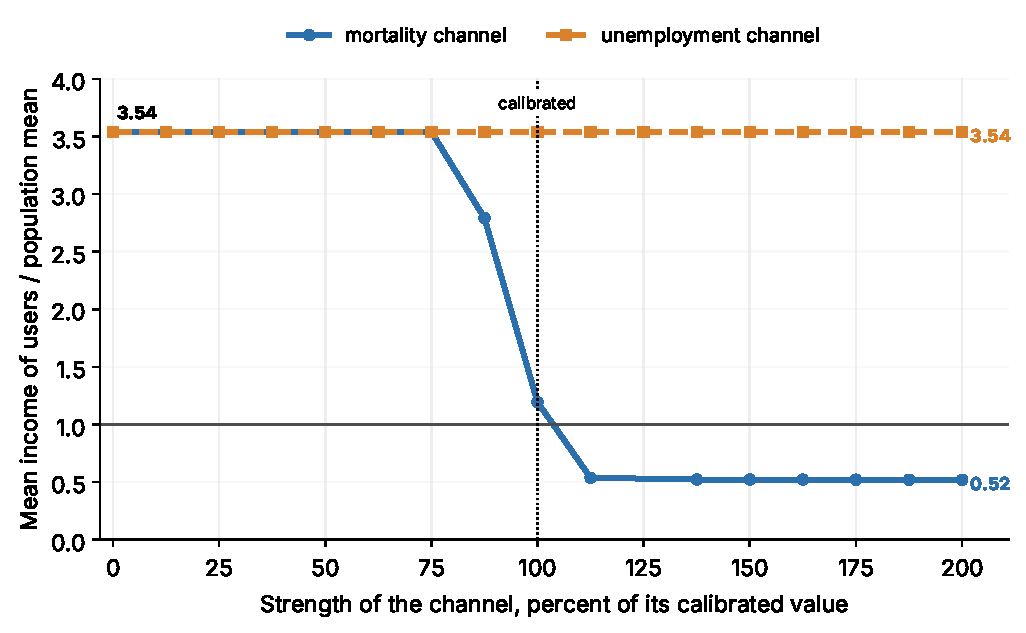
\includegraphics[width=0.62\textwidth]{figures/stylized_who_uses.pdf}
\caption{What it takes to reverse the income gradient in drug use}
\label{fig:who}
\notes{0.62\textwidth}{Note: stage 1, the model without the child. Each curve
scales one channel with the other switched off, so both start from the economy with no
consequences of a SUD. The vertical axis is average income of users over the
population average, and $b$ is recalibrated at every point so that participation is
the calibrated $8.92$ percent. The black dotted line marks the calibrated strength; everything to
the right of it is extrapolation.}
\end{figure}

The result is sharper than the statement that mortality matters more. On its own,
the mortality channel takes the income ratio from 3.54 with nothing switched on
down to 1.24 at its calibrated strength, and falls further to
0.52 as it continues to rise to $200$ percent of its calibrated
value.
What mortality destroys is a continuation value,
and a household only stops using when the expected loss of that value exceeds what
the drug is worth to it.

In contrast, the unemployment channel does not reverse the gradient at all: on its
own it leaves users at 3.54 times average income at its calibrated strength,
against 3.54 with nothing switched on, and at $200$ percent they
are still at 3.54. A resource penalty does not produce the concentration of
drug use at the bottom.

Why should the two channels differ at all, when in both the disorder
punishes the household? Because the cost of only one of them rises with the household's income. A job the disorder costs is not
covered by income support, so it drops the household to the same floor regardless of what it was earning. What it
has left is just food assistance, whatever it saved and, under Housing First, a voucher
if it draws one. Because risk aversion is above
one, utility has a ceiling, so how much a household loses in that fall stops growing with
its income: two households well above the floor lose about the same, even if one earns
twice as much as the other. The unemployment channel is therefore close to a flat charge
on using, the same for every household that would use. It changes how many use, which
the recalibration of $b$ undoes, but not which households do. On the other hand, buying $v$ units costs a rich household almost
nothing in terms of utility and a poor household a great deal, so the utility
price of using \emph{falls} as income rises, and that, combined with the bounded loss from acquiring a SUD, is what puts use at the top
to begin with.

Mortality is a different object. What it destroys is the whole
continuation value: the consumption of a life still to be lived, and $\aleph$,
the value of being alive at all, which does not shrink as consumption does. The value of life
rises with permanent income, so the expected cost of using rises with
income at the same time as its utility price falls. Past a point the two cross,
and it is the rich who stop first. The reversal therefore happens because the mortality
penalty rises quickly with income. The household with more to
lose loses more, and loses disproportionally more than it gains from drugs.

%======================================================================
\subsection{How does housing assistance shape the drug use decision?}\label{sec:mh}

The two forces of question 2, moral hazard and the value of life, can be separated exactly, because they differ in
what happens to a household that uses. Under Treatment First the voucher is
withdrawn from any household that violates the sobriety condition, so only the
value-of-life force operates. Under Housing First it is not, so both channels
operate. Comparing the two policies at the same generosity therefore isolates
the moral hazard force, and comparing Treatment First with no programme at all
isolates the value-of-life force.

Panels A and B of Table~\ref{tab:stage1} put numbers on both, in the baseline of stage 1. With no
programme at all, $7.62$ percent of households use. Treatment First takes that down to $4.19$ percent, a
value-of-life force that reduces drug use by $3.43$ percentage points.
Switching to Housing First then raises it even higher than before a programme existed, to
$8.92$ percent, so the moral hazard force raises drug use by $4.73$
percentage points and the
net effect of Housing First is a $1.30$ percentage point increase in drug use relative to
no vouchers at all. Both comparisons here are between long-run steady states, each the rest point of
the economy under a policy that has always been in place. Both forces are
first order and they work against each other, which is the central feature of
the problem. Anyone asserting that housing the homeless must increase drug use,
or must reduce it, is making a quantitative claim that needs to be tested.

The SUD rate follows participation one for one, since every user runs the same
risk: $3.15$ percent of households carry the disorder with no programme,
$1.73$ under Treatment First and $3.69$ under Housing First.
Homelessness falls under both programmes, from
$0.79$ percent to $0.56$ under Treatment First and
to $0.59$ under Housing First.

\begin{table}[!tb]
\centering
\caption{Stage 1: the two forces and the welfare of conditionality}\label{tab:stage1}
\sbox{\ntbox}{% Generated by code/stylized/stage_results.py from stage 1.
\footnotesize
\begin{tabular}{@{}lccc@{}}
\toprule
 & \textcolor{red}{None} & \textcolor{red}{TF} & \textcolor{red}{HF} \\
\midrule
\multicolumn{4}{@{}l}{\emph{Panel A. Outcomes, percent of households}} \\
\textcolor{red}{\quad Drug participation} & \textcolor{red}{9.49} & \textcolor{red}{1.53} & \textcolor{red}{9.02} \\
\textcolor{red}{\quad Carrying a SUD} & \textcolor{red}{3.925} & \textcolor{red}{0.632} & \textcolor{red}{3.729} \\
\textcolor{red}{\quad Homeless} & \textcolor{red}{1.378} & \textcolor{red}{0.998} & \textcolor{red}{1.014} \\
\addlinespace
\multicolumn{4}{@{}l}{\emph{Panel B. The two forces on participation, percentage points}} \\
\textcolor{red}{\quad Value of life, TF less none} &  & \textcolor{red}{$-7.96$} &  \\
\textcolor{red}{\quad Moral hazard, HF less TF} &  &  & \textcolor{red}{7.49} \\
\addlinespace
\multicolumn{4}{@{}l}{\emph{Panel C. Treatment First against Housing First}} \\
\textcolor{red}{\quad Households strictly worse off, percent} &  & \textcolor{red}{8.0} &  \\
\textcolor{red}{\quad Households strictly better off, percent} &  & \textcolor{red}{0.0} &  \\
\textcolor{red}{\quad CEV of those affected, percent} &  & \textcolor{red}{$-0.51$} &  \\
\textcolor{red}{\quad CEV of the population, percent} &  & \textcolor{red}{$-0.040$} &  \\
\bottomrule
\end{tabular}
}\usebox{\ntbox}
\tabnote{Note: stage 1, the model without the child and without the disamenity of
homelessness. None is no programme. Welfare changes are consumption-equivalent
variations: the proportional change in consumption, in every period and state, worth
as much as the difference in lifetime value, negative when Treatment First reduces welfare relative to
Housing First.}
\end{table}

%======================================================================
\subsection{Welfare}\label{sec:welfare}

\subsubsection{Without externalities, Housing First always wins}\label{sec:nox}

Sections~\ref{sec:who} and~\ref{sec:mh} established what each policy does to
behaviour. This section asks what each does to welfare, comparing the two at the
same generosity $\pi_V$, in the baseline of stage 1, where nothing a household does
lands on anybody else. Welfare is measured throughout as a consumption-equivalent
variation (CEV), set out formally in Section~\ref{sec:cev}. The policies differ only in the last indicator in
equation~\eqref{eq:vouch}, so Housing First transfers resources in a superset of
the states in which Treatment First does. The budget set is weakly larger in
every state and strictly larger in one, so a rational household with no commitment problems cannot be
worse off under Housing First:
\begin{equation}\label{eq:dom}
V_1(y;\ \text{HF},\ \pi_V) \;\ge\; V_1(y;\ \text{TF},\ \pi_V)
\qquad \text{for every } y,
\end{equation}
with equality exactly for households that never use under Housing First. Put the other way round, a
household under Housing First can reproduce its Treatment First outcome exactly
by not using: conditionality removes an option from a forward-looking optimiser
and gives nothing back. This is a dominance argument, not a calibrated result,
and no choice of parameters overturns it.

It follows that the moral hazard is not an inefficiency. Households here face the
true SUD hazard and make no mistakes, so the extra use Housing First
induces is not a wedge to be closed but a household optimally taking a risk it
is able to bear. The moral hazard force of Section~\ref{sec:mh} is a
statement about drug use and not about welfare.

Panel C of Table~\ref{tab:stage1} puts welfare numbers on it:
$9.4$ percent of households are strictly worse off under
Treatment First,\footnote{The share worse off is above the $8.92$
percent who use under Housing First, because a household that would use in only some of
its period 1 draws is worse off in full but counts in participation only in the draws in
which it uses.} none is better off, and those affected lose the equivalent of $0.17$ percent
of consumption. Those are the households that use under Housing First and
can draw a voucher: a household that never uses faces the same voucher rule under
both policies and is indifferent between them. 

A fixed budget does not rescue the welfare case for conditionality either. The two
programmes cost almost the same, $2.14$ percent of mean income per household under
Treatment First against $2.15$ percent under Housing First, so matching on cost
rather than on generosity would change nothing. Both programmes give a voucher to the same
share $\pi_V$ of eligible households, and Treatment First then denies it to those that fail the
sobriety condition, so it pays out less for that reason; the two costs are close because, in equilibrium under Treatment First, households are deterred, and thus few of
the households that draw a voucher fail the condition. Therefore, the case for conditionality in
this model has to come from elsewhere: from what a household's drug use does to
somebody else.

%======================================================================
\subsection{Stage 2: the child}\label{sec:kids}

Some of the externalities modelled in this paper are the ones imposed on the
children of households with a SUD. This stage adds the child, as the quantitative
model has it, and refits the model with the child in place.

\paragraph{The child in the household.} Each household raises one child
during its adulthood period. The child shares the household's consumption and housing
through the square-root equivalence scale $\xi$, while the drug only enters the utility of the parent, so the parent and the child hold different bundles,
\begin{equation}\label{eq:bundleskid}
X_P=\Big[\Big(\frac{c}{\xi}\Big)^{1-\gamma}\Big(\frac{h}{\xi}\Big)^{\gamma}\Big]^{1-\theta}(b+v)^{\theta},
\qquad
X_c=\Big[\Big(\frac{c}{\xi}\Big)^{1-\gamma}\Big(\frac{h}{\xi}\Big)^{\gamma}\Big]^{1-\theta}\,b^{\theta},
\end{equation}
and the parent's flow utility in period 1 becomes
\begin{equation}\label{eq:ukid}
u_1(c,h,v) \;=\; U(X_P)\;+\;\omega_c\,(\xi-1)\,U(X_c)\;+\;\aleph .
\end{equation}
The child consumes the household's consumption and housing but none of the drug, so
a parent's drug spending reaches it only by taking consumption and housing out of what
they share, and it counts as $\xi-1$ of the household against the scale. The weight $\omega_c$ is the
share of the child's utility that the parent takes into account. Without the drug and with
$\omega_c=1$, the first two terms are $U(X)+(\xi-1)\,U(X)=\xi\,U(X)$, the usual form, which
counts the household as $\xi$ adult equivalents: the parent as one and the child as the
remaining $\xi-1$. In period 2, when the parent moves into old age, the child leaves and the parent lives alone, $\xi=1$, and flow utility is that of~\eqref{eq:u}.

\paragraph{The child leaves.} At the end of period 1 the child leaves the
household and becomes an adult, entering period 1 of its own life, with its own child living with it. Its productivity
is correlated with its parent's, and it is permanently reduced if the parent acquired the disorder while the
child lived with it,
\begin{equation}\label{eq:kids}
\log y_{\text{child}} \;=\; \rho\log y+(1-\rho)\log\bar y+\varepsilon
-\delta_d\,\mathbf{1}\{d'=1\},
\qquad \varepsilon\sim\mathcal N\big(0,\,(1-\rho^2)\,\sigma_y^2\big),
\end{equation}
where $\rho$ is the persistence of productivity across generations, $\bar y$ is
average income, the variance of $\varepsilon$ keeps the spread of productivity the same
in every generation, and $\delta_d$ is the penalty for the parent's disorder. 

\paragraph{The parent's problem.} The child enters the parent's problem
twice, once for each part of its life. In childhood it is the second term
of~\eqref{eq:ukid}. As an adult it is the continuation value $D(y)$, what the parent's
disorder costs its child in the child's own lifetime value,
\begin{equation}\label{eq:damage}
D(y)\;=\;\mathbb{E}\big[\bar V_1(y_{\text{child}})\,\big|\,y,\,d'=0\big]
-\mathbb{E}\big[\bar V_1(y_{\text{child}})\,\big|\,y,\,d'=1\big]\;\ge\;0,
\end{equation}
where $\bar V_1$ is the value of entering period 1, before its draws, at the child's
productivity from~\eqref{eq:kids}. $D(y)$ captures the direct impact of the parent's SUD on
its child's utility, which runs through the child's earnings. It enters as a difference and not
a level, so it costs the parent nothing unless its use makes the disorder possible. The period 1 problem in~\eqref{eq:v1} in Section~\ref{sec:problem} then becomes
\begin{equation}\label{eq:v1kid}
V_1(y,e,\eta) = \max_{\{k,\,v \ge 0,\,a' \ge 0\}}
\Big\{ u_1(c,h_k,v)
+ \beta\, \mathbb{E}_{d'}\Big[\phi(d')\,V_2(a',y,d')\Big]
-\ \beta\,\omega_c\,\pi(v)\,D(y) \Big\}.
\end{equation}
$\omega_c$ multiplies both child terms. A planner who counted the child
fully would put a weight of one on both, so what the parent leaves out, $1-\omega_c$ of
the child's terms, is the externality on the child. $D$ is weighted by $\pi(v)$, the chance that the use turns into a disorder. $V_1$ depends on $D$ through the
parent's problem and $D$ on $V_1$ through the child's, so the two are solved as a
fixed point.

\paragraph{Why income, and not susceptibility.} The penalty runs through
income rather than through anything the child inherits about the drug.
Letting the child inherit a greater
susceptibility, a higher $\pi_d$, fails. A child facing a
higher chance of converting use into a SUD optimally uses \emph{less} ex ante, which is at odds with the
data: children of parents with a SUD are \emph{more} likely to use, not less.

In contrast to the above, income works on both counts, and it works through the channels explored in
Section~\ref{sec:who}: lower permanent income is unambiguously bad to receive,
and this model already puts users at the bottom, so a child born poorer is
mechanically more likely to use, which is aligned with the data. It is also
supported by the empirical evidence reviewed in Section~\ref{sec:literature}. The income
gradient does the whole job, so the model transmits a SUD across generations
without the child inheriting any greater susceptibility to the disorder.

\paragraph{Calibrating the child.} With the child added, $\xi$, $\rho$, $\delta_d$ and
$\omega_c$ need to be calibrated as well. I set $\xi$ to $\sqrt2$, the square-root scale for a household of two (OECD, 2013). The
persistence of productivity across generations, $\rho$, \new{is set to} $0.50$, within the range of the
intergenerational elasticities of earnings in Section~\ref{sec:literature}. The penalty
$\delta_d$ \new{is assigned the value} $0.27$ in logs \new{to give} the $24$ percent earnings loss Nilsson (2017)
measures for children exposed in utero to a temporary Swedish policy that let grocery
stores in two regions sell strong beer, which made alcohol easier to buy during pregnancy.
The parent's weight on its child $\omega_c$ is fitted so that switching the child's terms
off, with every other parameter held, raises drug use by $18.3$ percent, consistent
with adults without children in NSDUH 2024 using $18.3$ percent more than parents. Every other stage 1 parameter is refitted with the child in place, and
Table~\ref{tab:int} reports both.

\paragraph{The optimal level of drug use.} To examine what the optimal degree of
drug use and SUD is, one can set the weight a parent puts on its child to one,
$\omega_c=1$, so that a parent counts its child fully, with nothing else changed and the
programme left as it is. In this case, no parent uses at all: participation and the SUD rate
both fall to $0.00$ percent, and homelessness to $0.55$ percent.

\paragraph{Treatment First with the child counted.} Counting the child's utility in
welfare, as Section~\ref{sec:cev} describes, a newborn is better off under Treatment First
than under Housing First, by $0.46$ percent of
lifetime consumption in the long run. The dominance of Section~\ref{sec:nox} still holds
for the parent's own choices; what reverses the ranking is what those choices do to the
child. Treatment First cuts participation from $8.83$ to $7.00$
percent and the share carrying the disorder from $4.00$ to $2.96$
percent, so fewer children enter adult life with the penalty, and the gain is
$0.22$ percent in childhood, because parents spend more of their
resources on them instead of on drugs, and $0.24$ percent in adult
life, where the child enters with a better draw. Homelessness is lower too, $0.56$ against
$0.57$ percent, because fewer households have a SUD and lose their jobs
with no income support, and fewer are themselves poor for having been born to a
parent with the disorder, so their income is higher.

%======================================================================
\subsection{The transition}\label{sec:trans}

Comparing rest points hides a key tradeoff. Normally, the debate sees Treatment First as taking immediately and
giving back only later\new{. In this model, this happens too}: at implementation a household with a SUD can do nothing about
its condition but loses its voucher, and it \new{is} then at a higher risk of homelessness,
whereas lower substance use pays off only for the
generations after it. \new{However, in this model,} a reduction in drug use can also benefit
children at once: the children of parents who use drugs but do not yet have a SUD escape
the earnings penalty \new{and enjoy larger consumption} if their parents respond to the policy change by stopping.

The reform moves the programme from Housing First to Treatment First at the same
$\pi_V=0.27$, in the model with the child, and every generation alive
when it lands is counted, each over its own remaining life and against what the old
rule would have given it. Figure~\ref{fig:trans} shows the path: drug use, the
disorder and homelessness of each generation as adults, from the adults at the reform on,
against the Housing First rest point, and the welfare of every generation: the old and
the adults alive at the reform, their children, and the cohorts born after them.

The old, in their second period, chose under the old rule,
carry whatever disorder that choice left them and cannot recover in a terminal period;
conditionality now withdraws the voucher from those carrying one, and they lose
$0.07$ percent of consumption, with $0.74$ percent of them
homeless against $0.73$ under the old rule. The adults, in their first
period with their children at home, who were born into the old distribution, choose
under the new rule; they lose $0.018$ percent over their adult lives,
the price of an option removed.

Their children, the first cohort born into the reform, gain
$0.36$ percent: $0.24$ in adult life, since they are the first to
enter it with the draws of parents who chose under Treatment First, and $0.11$ in childhood, against the
$0.22$ that childhood contributes in the long run, since the parents they grow up with were themselves born
into the penalised distribution. From the second cohort on the chain is at its
new rest point and every cohort gains the long-run $0.46$ percent. The cost
falls on the adults and the old alive at the reform, and the benefit on the children
born at the reform and, even more, on every cohort born after them.

\begin{figure}[!tb]
\centering
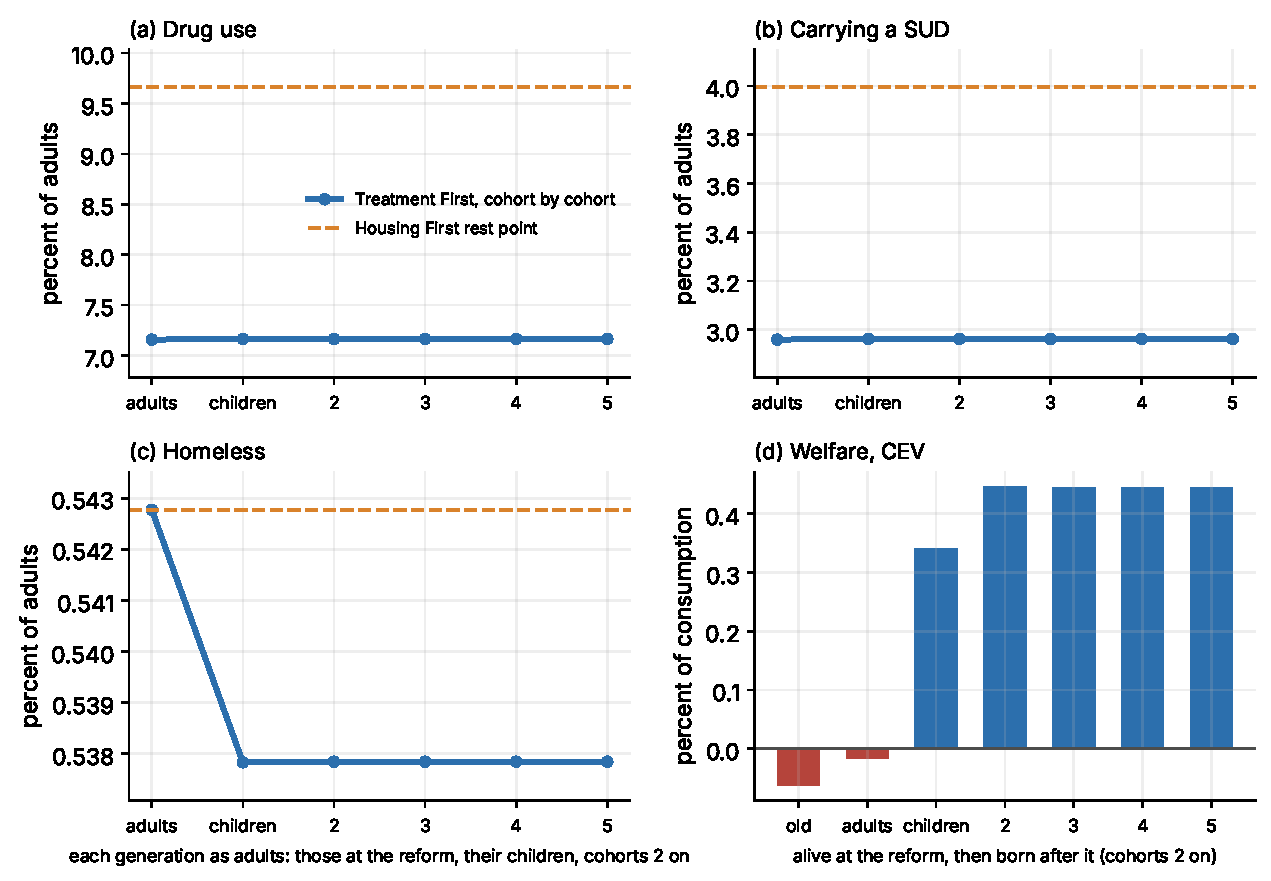
\includegraphics[width=\textwidth]{figures/stylized_transition.pdf}
\caption{The transition from Housing First to Treatment First}\label{fig:trans}
\notes{\textwidth}{Note: the model with the child. Panels (a) to (c) are each
generation as adults, in their first period: the adults at the reform, who were born into
the Housing First distribution and choose under Treatment First, their children, and the
cohorts born after them, \new{when they become adults,} to the fifth; the solid blue line is Treatment First,
cohort by cohort, and the dashed orange line is the Housing First rest point. Panel (d)
is each generation's CEV against Housing First: the old and the adults alive at the
reform over the rest of their lives, and their children and every cohort born after them
over their whole lives.}
\end{figure}

%======================================================================
\subsection{Stage 3: the disamenity of homelessness}\label{sec:kx}

The second externality lands on everybody. Each household's flow utility falls by
$\kappa_x H$, where $H$ is the share of households that is homeless, which every
household takes as given, so the term moves no choice and the calibration of stage 2
stands unchanged. It enters welfare only, and the child
bears it like everyone else, once for each period.

$\kappa_x$ is solved inside the model from the willingness to pay for ending
homelessness in the contingent valuation of Loubi\`ere et al.\ (2020), $0.2$
percent of income. Households in the model spend $73$ percent of their income
on consumption, so \new{$0.2$ percent of income translates to} $0.27$ percent of consumption. $\kappa_x$ is the
disamenity per unit of homelessness, in utils per period alive, that costs an adult in
the stage 2 economy as much over its adult life as giving up $0.27$ percent of
its consumption in every period. That gives
$\kappa_x=1.31$. Because the two policies differ little in homelessness, it changes essentially nothing about the welfare gain from Treatment First, which remains at
$0.46$ percent of lifetime consumption.

%======================================================================
\section{The quantitative model}\label{sec:full}

\new{This section describes the model the paper's numbers come from. It is the stylized
model of Section~\ref{sec:stylized} with a life cycle of annual periods and the pieces
that model leaves out: income risk over working life, retirement, recovery and
treatment, SMI, a government budget and a drug market. Notation follows
Section~\ref{sec:stylized} wherever the two models share an object: $\gamma$ and
$\theta$ are the housing and drug weights in both, $b$ is the same Stone-Geary
shifter, $\aleph$ the same flow value of being alive, $\xi$ the same equivalence
scale, $\omega_c$ the same weight on the child, $\rho$ and $\delta_d$ the same
persistence of productivity and penalty, $\psi_{ui}$ and $\bar y$ the same replacement
rate and earnings cap, $\kappa_x$ the same disamenity, and $\beta$ is the discount
factor. The values are in Section~\ref{sec:fullcal}.}

\subsection{Demographics and the state and choice sets}

\new{Households enter the economy as adults at model age $j=1$, which is age 26, live
at most $J$ annual periods, work while $j<J_R$ and are retired from $J_R$. Each has a
child, which lives in the household for the first $J_K$ years of its adult life, until
age 50, and then leaves. Each period a cohort of unit mass enters at $j=1$, made up of
the grown children of the households that died, in proportion to their parents'
deaths, so the mass of households is constant in a stationary equilibrium. The individual state is
\begin{equation}\label{eq:fstate}
s=(a,\,y,\,e,\,d,\,m,\,\eta)\in
\mathcal A\times\mathcal Y_j\times\{1,2,3\}\times\{0,1,2\}\times\{0,1\}\times\{0,1,2\},
\end{equation}
where $a$ denotes assets, $y$ productivity, $e$ employment status, $d$ the SUD, $m$
SMI and $\eta$ the household's standing with the voucher programme. The SUD takes
three values because the parent's valuation of its child's prospects depends on its
history and not only on its present (Section~\ref{sec:fproblem}): $d=0$ for a household that has never carried the disorder, $d=1$ for
one that carried it and has recovered, and $d=2$ for one that carries it now. The
voucher state is $\eta=0$ without a voucher, $\eta=1$ holding one, and $\eta=2$
excluded from the programme after failing Treatment First's condition.}

\new{Each period the household chooses
\begin{equation}\label{eq:fchoice}
\big(h',\,v,\,\tau,\,a'\big)\in
\{h_1,h_2,h_3,h_4\}\times\mathbb R_+\times\{0,1\}\times\mathcal A ,
\end{equation}
where $h'$ is the dwelling, of which $h_1$ is a shelter, $v$ drug use, $\tau$ SUD
treatment, available only to a household that carries the disorder, and $a'$ next
period's assets. Labour supply is not a choice: a household that has a job works it.}

\subsection{Preferences}\label{sec:fprefs}

\new{Flow utility is the stylized model's, with the child present for the first $J_K$
years. Consumption $c$ and housing $h'$ are shared through the square-root equivalence
scale $\xi_j$, which is $\sqrt 2$ while the child is at home and one after, and the
drug is the parent's alone, so the parent and the child hold the bundles
\begin{equation}\label{eq:fbundles}
X_P=\Big[\Big(\frac{c}{\xi_j}\Big)^{1-\gamma}\Big(\frac{h'}{\xi_j}\Big)^{\gamma}\Big]^{1-\theta}(b+v)^{\theta},
\qquad
X_K=\Big[\Big(\frac{c}{\xi_j}\Big)^{1-\gamma}\Big(\frac{h'}{\xi_j}\Big)^{\gamma}\Big]^{1-\theta}b^{\theta},
\end{equation}
and period utility is
\begin{equation}\label{eq:futil}
u\big(c,h',v,\tau\big) \;=\; U(X_P)\;+\;\omega_c\,(\xi_j-1)\,U(X_K)\;+\;\aleph\;-\;\tau\,\bar\tau^{u},
\qquad U(X)=\frac{X^{1-\sigma}}{1-\sigma}.
\end{equation}
$\gamma$ is housing's share of the non-drug bundle and $\theta$ the drug's share of
the whole, $\sigma$ is the coefficient of relative risk aversion, $\aleph$ is the flow
value of being alive, counted once per household, and $\bar\tau^{u}$ is the utility
cost of a year in treatment. The child's term is its own flow utility, weighted by
$\omega_c$ and counted as $\xi_j-1$ of the household; it gets none of the drug, so a
parent's drug spending reaches it only through the consumption and housing they
share. After $J_K$ the child has left, $\xi_j=1$, and the term is gone.}

\new{Aggregate homelessness $H$ carries the disamenity $\kappa_x H$ for every household,
which is what makes homelessness an externality for everyone rather than only a
private misfortune. It enters every household's welfare and no household's decision:
each takes $H$ as given, and the term is left out of the problem it solves.
Section~\ref{sec:fleftout} takes up its size.}

\subsection{Income, taxes and transfers}\label{sec:ftaxes}

\paragraph{\new{Productivity.}} \new{Log productivity follows a persistent process over
working life, $z_{j+1}=\rho_z z_j+\upsilon_{j+1}$ with $\upsilon\sim\mathcal N(0,\sigma_\upsilon^2)$,
discretised on a grid whose width grows with the variance of $z$ at each age, and it is
frozen at its last working value in retirement. Earnings on the job are
$y\,\varepsilon(j)$, with $y=e^{z}$ normalised so that productivity averages one at
entry and $\varepsilon(j)$ the deterministic age profile. The lowest node of the grid is
held at a fixed level at every age, with the others rescaled to keep the mean. A
household's productivity at entry is its inheritance from its parent, set out in
Section~\ref{sec:fnewbornsec}; its spread combines $\sigma_\upsilon$ with a persistent
component drawn at entry, and a child entering with the penalty of that section is on a
separate block of the grid, the base grid scaled down for life.}

\paragraph{\new{Gross income.}} \new{It depends on age and employment,
\begin{equation}\label{eq:fincome}
Y(j,y,e)=
\begin{cases}
y\,\varepsilon(j) & j<J_{R},\ e=1 \quad\text{(employed)}\\[2pt]
\psi_{ui}\,\min\{y\,\varepsilon(j),\ \bar y\} & j<J_{R},\ e=2 \quad\text{(insured, first year out of work)}\\[2pt]
0 & j<J_{R},\ e=3 \quad\text{(out of work, uninsured)}\\[2pt]
S(y) & j\ge J_{R} \quad\text{(retired)} .
\end{cases}
\end{equation}
Unemployment insurance (UI) replaces the share $\psi_{ui}$ of earnings on a base capped
at average earnings $\bar y$, and it is paid for one year only, to the share $p_{ui}$
of separations that are insured. Social security $S(y)$ follows the statutory formula:
a primary insurance amount that replaces declining shares of the household's
productivity at its last working age, capped, between two bend points, with the
Supplemental Security Income (SSI) payment as a floor, all in units in which
productivity averages one at entry. The SUD and SMI do not
cut earnings on the job; they act on whether there is a job at all, through the
employment transitions below.}

\paragraph{\new{Taxes.}} \new{Gross income is taxed with the Heathcote et al.\ (2017) function
and capital income at a flat rate,
\begin{equation}\label{eq:ftax}
y^{n}=\min\big\{Y,\ \tau_{\ell}\,Y^{\varphi}\big\}\;+\;(1-\tau_k)\,r\,a ,
\end{equation}
with $\tau_{\ell}$ the level, $1-\varphi$ the progressivity, $\tau_k$ the capital
income tax and $r$ the exogenous interest rate on savings.}

\paragraph{\new{Transfers.}} \new{Food assistance pays the maximum allotment $\underline c$ less
the share $\varrho$ of income, the statutory taper without the statute's deductions or
its schedule by household size, and the voucher pays a holder that is eligible this
period the rent on the dwelling above a tenant contribution of $\kappa_r$ of income, up
to the fair market rent,
\begin{equation}\label{eq:ftrans}
\begin{aligned}
F&=\max\big\{0,\ \underline c-\varrho\,\hat y\big\},\\
V\!ch&=\mathbf{1}\{\eta=1\}\,\mathbf{1}\{\hat y<\kappa_V y^{\text{med}}\}\,\mathbf{1}\{h'\neq h_1\}\,
\min\Big\{\max\{0,\ p_r h'-\kappa_r\hat y\},\ \max\{0,\ \mathit{FMR}-\kappa_r\hat y\}\Big\},
\end{aligned}
\end{equation}
where $\hat y=Y+r\max\{a,0\}$ is the income both programmes are means-tested on,
$\kappa_V$ and median income $y^{\text{med}}$ are the eligibility rule
of~\eqref{eq:felig}, and $\mathit{FMR}$ is the average rent paid by housed renters in
the benchmark. A voucher
holder in a shelter keeps the voucher and is paid nothing until it rents again. Each
entering household receives a one-time transfer $T_0$ from the government, and the
government collects the estates of the dead.}

\subsection{The budget constraint}

\new{\begin{equation}\label{eq:fbudget}
c+p_v v+a' \;=\; y^{n}+a+T_0\mathbf{1}\{j=1\}\;-\;p_r\, h'\,\mathbf{1}\{h'\neq h_1\}\;+\;V\!ch+F,
\qquad c\ge F,\ v\ge0,\ a'\ge0 .
\end{equation}
Food assistance is paid in kind, so it cannot fund the drug, the rent or saving. The
drug price is $p_v$ and the rent per unit of housing $p_r$, held at its benchmark value
in every simulation. Treatment costs utility and no money.}

\subsection{Housing and the homelessness loop}

\new{Housing is the four point grid of~\eqref{eq:fchoice}: $h_1$ is literal
homelessness, sleeping rough or in an emergency shelter, which is free, and $h_2<h_3<h_4$
are three rental sizes, the larger two fixed multiples of the smallest. In the last
years of life the shelter is not available, for the same reason the drug has an
initiation age (Section~\ref{sec:fdrug}): too little life remains for its costs to
bind.}

\new{Homelessness then enters three separate equations: survival~\eqref{eq:fsurv}, the
employment transitions~\eqref{eq:femp} and the SUD recovery hazard~\eqref{eq:frecover}.
It raises mortality, worsens both employment margins and lowers the chance of
recovering from the SUD. SMI is the one thing it does not reach, for the reason given
in Section~\ref{sec:fsmi}.}

\subsection{Drug use, the SUD, recovery and treatment}\label{sec:fdrug}

\new{A household that does not carry the disorder, $d\in\{0,1\}$, and uses any
quantity acquires it with probability $\pi_d$,
\begin{equation}\label{eq:fd}
\Pr(d'=2\mid d\neq 2,\,v)=\pi_d\,\mathbf{1}\{v>0\},
\end{equation}
so the risk is a cost of using at all and not of the dose, and a household that has
recovered can acquire the disorder again. A household may begin using only up to an
age $J_E$.\footnote{Without it there is little consequence at old ages to using: too
little life remains for the disorder to damage, so the model produces too much of
it.} A household with the SUD recovers, to $d=1$, with probability
\begin{equation}\label{eq:frecover}
\pi_r(h',m,\tau)=\min\Big\{1,\ \bar\pi_r\,
\mu_H^{\mathbf{1}\{h'=h_1\}}\,\mu_m^{\mathbf{1}\{m=1\}}\,g^{\tau}\Big\},
\end{equation}
with $\bar\pi_r$ the baseline annual chance of recovering while housed, without SMI
and untreated, and three multipliers on it: $\mu_H<1$, which means that recovery is
harder in a shelter, $\mu_m<1$, which means that it is harder with SMI, and $g>1$,
which means that it is more likely in treatment.}

\new{$\mu_H$ is how housing acts on drug use here, and it is worth being exact about what
that claim is and is not. Housing does not change what a household wants: flow utility
is the same function of $(c,h',v)$ housed or not. What housing changes is the chance of
getting out of the disorder once it is carried. Milby et al.\ (2005) randomised
cocaine-dependent homeless adults into arms differing in housing and measured weeks of
abstinence, so the ratio between arms identifies $\mu_H$.}

\new{Treatment $\tau$ is a \emph{choice}, taken at the utility cost $\bar\tau^u$
in~\eqref{eq:futil}, and $g$ is the only thing it buys. It does not stop the household
using, it does not remove the excess mortality of the disorder while it lasts, and it
does not exempt the household from Treatment First's condition, since a household in
treatment still carries the disorder.}

\subsection{Serious mental illness}\label{sec:fsmi}

\new{$m$ is a two state Markov chain representing SMI, whose prevalence is
a small share of adults, defined by substantial functional impairment, rather than any
mental illness, which is roughly a quarter of adults and includes mild anxiety. Onset
has an age profile $\varsigma_m(j)$, the onset implied by the prevalence of SMI by age
in NSDUH 2024, normalised to one at age $26$, and a level $\omega_m$, and a household that
carries the disorder faces $\iota>1$ times the rate,
\begin{equation}\label{eq:fonset}
\Pr(m'=1\mid m=0,d)=\min\big\{1,\ \omega_m\,\varsigma_m(j)\,\iota^{\mathbf{1}\{d=2\}}\big\},
\qquad
\Pr(m'=0\mid m=1)=\lambda_m .
\end{equation}
That last channel runs in the direction the evidence supports: substance induced
psychosis converts to schizophrenia or bipolar disorder at a pooled rate near a quarter
(Murrie et al., 2020), and in the Danish registers any SUD predicts conversion to
schizophrenia with a hazard ratio of $1.34$, opioid use disorder $2.74$ (Nielsen et
al., 2017).}

\new{SMI then affects three objects: both employment margins, through~\eqref{eq:femp},
mortality, through~\eqref{eq:fsurv}, and the SUD recovery hazard, through $\mu_m$
in~\eqref{eq:frecover}. It does not change the utility function or earnings on the job.}

\new{The SMI chain does \emph{not} depend on housing, and that is a finding in the data
rather than an omission. In the At Home / Chez Soi randomised trial, $1{,}198$ homeless
adults with SMI across four cities, assignment to housing with intensive case
management produced no detectable effect on symptom severity at any wave, while
producing large effects on housing stability, its primary outcome. Making the channel
housing dependent would mean adding a mechanism the best available trial looked for
and did not find.}

\subsection{What the SUD, SMI, and homelessness cost}\label{sec:fcosts}

\paragraph{\new{Death risk.}}\label{sec:fdeath} \new{Write $\bar q_j$ for the baseline
probability of dying at age $j$, from the Social Security Administration (SSA) period
life table, and
$q^{\,0}_j(h')=\min\{1,\kappa_{\phi H}^{\mathbf{1}\{h'=h_1\}}\,\bar q_j\}$ and
$q^{\,1}_j(h')=\min\{1,\kappa_{\phi d}\,\kappa_{\phi H}^{\mathbf{1}\{h'=h_1\}}\,\bar q_j\}$
for the probability without and with the disorder. The probability of dying is then
\begin{equation}\label{eq:fsurv}
1-\phi(j,h',d,m)=\min\Big\{1,\ \kappa_{\phi m}^{\mathbf{1}\{m=1\}}\,q^{\,0}_j(h')
+\mathbf{1}\{d=2\}\big[q^{\,1}_j(h')-q^{\,0}_j(h')\big]\Big\},
\end{equation}
so $\kappa_{\phi H}$ multiplies the death probability of a household in a shelter,
$\kappa_{\phi d}$ that of a household carrying the disorder, and $\kappa_{\phi m}$ the
baseline risk of a household with SMI, to which the excess risk of the disorder is
added. The multipliers act on the annual probability of dying, which at an annual
frequency is close to the hazard whose ratios the sources report, and the cap keeps it a
probability. The disorder kills
whether or not it is being treated: the excess mortality of a SUD is overwhelmingly a
mortality of use, poisoning above all, and treatment in the model does not stop use.
\footnote{In the data, the meta-analyses of mortality among people using extramedical
opioids report overdose as the largest single contributor to the excess (Larney et al.,
2020; Degenhardt et al., 2011), and in the Centers for Disease Control and Prevention
(CDC) WONDER database drug poisoning alone accounts for about a fifth of all deaths at
ages 25 to 44, which is the moment Section~\ref{sec:fvalid} reports the model
against.}}

\paragraph{\new{Unemployment risk.}} \new{A job is lost with probability $\pi^{eu}$ and found
with probability $\pi^{ue}$,
\begin{equation}\label{eq:femp}
\pi^{eu}=\min\Big\{1,\ \bar\pi^{eu}\,a(y)\,
\kappa^{eu}_{m}{}^{\mathbf{1}\{m'=1\}}(1+\kappa_{H})^{\mathbf{1}\{h'=h_1\}}\Big\},
\qquad
\pi^{ue}=\min\Big\{1,\ \frac{\bar\pi^{ue}\,(1-\kappa_{H})^{\mathbf{1}\{h'=h_1\}}}
{\kappa^{ue}_{d}{}^{\mathbf{1}\{d'=2\}}\,\kappa^{ue}_{m}{}^{\mathbf{1}\{m'=1\}}}\Big\},
\end{equation}
with $\bar\pi^{eu}$ and $\bar\pi^{ue}$ the baseline separation and job finding rates,
$a(y)$ a factor that makes separations likelier at low productivity, in line with the
unemployment rates of the education groups the productivity grid spans, the multiplier
$\kappa^{eu}_{m}$ making a job likelier to lose with SMI, and the divisors
$\kappa^{ue}_{d}$ and $\kappa^{ue}_{m}$ making one harder to find with the SUD and with
SMI. The SUD does not raise separations. $\kappa_{H}$ does both for a household in a
shelter.}

\paragraph{\new{The child's productivity penalty.}} \new{A child whose parent carries the
disorder in the period the parent dies enters the economy with its productivity lowered
by the proportion $\delta_d$ in~\eqref{eq:fnewborn}, and the penalty stays with the
child for life. There is no penalty for a parent's homelessness. The parent's own
problem prices the penalty on a different event, set out in
Section~\ref{sec:fproblem}. The penalty is a risk to the
parent's own objective only to the extent that $\omega_c$ is positive, so it is the one
risk here that carries an externality rather than a pure personal cost, which is what
makes it a candidate for policy in a way that mortality and unemployment risk, both
fully internalised, do not.}

\subsection{The voucher and the two policies}\label{sec:fvoucher}

\new{A household is eligible for a voucher while its income is below the share
$\kappa_V$ of median income,
\begin{equation}\label{eq:felig}
\hat y\;<\;\kappa_V\,y^{\text{med}},
\end{equation}
with $\hat y$ the income of~\eqref{eq:ftrans}. A holder keeps its voucher while it is
eligible, so unlike Section~\ref{sec:support} the voucher is persistent rather than
redrawn each period, and an eligible household without one draws one with probability
$\pi_V$. Under Housing First that is the whole rule.}

\new{Under Treatment First the programme is conditional. A household fails the condition if
it uses or carries the disorder, $v>0$ or $d=2$, whether or not it is in treatment. A
holder that fails it is detected with probability $p_{\text{det}}$, and so is an
applicant that fails it when it draws a voucher, and a household that is detected is
excluded, $\eta'=2$. An excluded household cannot draw a voucher
whatever its income, and it returns to the lottery, $\eta'=0$, with probability
$\psi_x$ each year. The test acts on next period's standing, so the voucher a household
holds this period pays out this period. It reaches only households that are income
eligible, and the government pays $c_{\text{test}}$ for each one it tests.}

\new{This means that in contrast to Section~\ref{sec:mh}, enforcement here need not be
perfect: with $p_{\text{det}}<1$ some who fail the condition keep their voucher. None of
$p_{\text{det}}$, $\psi_x$ and $c_{\text{test}}$ binds in the benchmark, where no voucher
is conditional, so all three are set with the experiment in
Section~\ref{sec:experiments} rather than in the calibration.}

\subsection{The shocks, collected}\label{sec:fshocks}

\new{Conditional on the state and the choices, next period's state is drawn in five
transitions, which are independent given the state except that employment depends on
next period's SUD and SMI and on the dwelling $h'$ through~\eqref{eq:femp}:}

\paragraph{\new{Productivity $y$.}} \new{By the process of Section~\ref{sec:ftaxes} while
working, and unchanged in retirement.}

\paragraph{\new{Employment $e$.}} \new{A household that loses its job is insured with probability
$p_{ui}$, for one year. With $\pi^{ue}$ and $\pi^{eu}$ from~\eqref{eq:femp},
\begin{equation}\label{eq:fetrans}
e=1\ \longrightarrow
\begin{cases}
e'=1 & \text{w.p. } 1-\pi^{eu}\\
e'=2 & \text{w.p. } p_{ui}\,\pi^{eu}\\
e'=3 & \text{w.p. } (1-p_{ui})\,\pi^{eu}
\end{cases}
\qquad
e\in\{2,3\}\ \longrightarrow
\begin{cases}
e'=1 & \text{w.p. } \pi^{ue}\\
e'=3 & \text{w.p. } 1-\pi^{ue}.
\end{cases}
\end{equation}
State $2$ is reachable only from employment and never from itself, so the insured are
in it for the first year out of work and then move to state $3$, which pays nothing.}

\paragraph{\new{The SUD $d$.}} \new{By~\eqref{eq:fd} if $d\neq2$ and~\eqref{eq:frecover} if
$d=2$, conditioning on the chosen $v$, $h'$ and $\tau$ and on $m$.}

\paragraph{\new{Mental illness $m$.}} \new{By~\eqref{eq:fonset}, conditioning on $d$ and age.}

\paragraph{\new{The voucher $\eta$.}} \new{By~\eqref{eq:felig} and the rule of
Section~\ref{sec:fvoucher}, conditioning on this period's eligibility and, under
Treatment First, on the chosen $v$ and the state $d$.}

\new{Write $\Gamma\big(s'\mid s,\,h',v,\tau\big)$ for their joint law, which is
the object the expectation in~\eqref{eq:fbellman} is taken against.}

\subsection{The household's dynamic problem}\label{sec:fproblem}

\new{Putting it together, for $j=1,\dots,J$ and with $V(J{+}1,\cdot)=0$,
\begin{equation}\label{eq:fbellman}
\begin{aligned}
V(j,s)=\max_{\{h',\,v,\,\tau,\,a'\}}\ \Bigg\{\
&U(X_P)+\omega_c(\xi_j-1)\,U(X_K)+\aleph-\tau\bar\tau^{u}\\[2pt]
&+\ \beta\,\phi(j,h',d,m)\!\int_{\mathcal S}\! V(j{+}1,s')\,
\Gamma\big(\mathrm{d}s'\mid s,h',v,\tau\big)\\[2pt]
&-\ \beta\,\chi_j\,\omega_c\,\max\big\{\mathbf{1}\{d\ge1\},\,\mathbf{1}\{v>0\}\big\}\,D(y)\Bigg\},
\qquad
\chi_j=\begin{cases}1-\phi(j,h',d,m) & j<J_K\\ 1 & j=J_K\\ 0 & j>J_K,\end{cases}
\end{aligned}
\end{equation}
subject to the budget~\eqref{eq:fbudget}, the income and transfer
rules~\eqref{eq:fincome} to~\eqref{eq:ftrans}, and the restrictions that treatment is
available only to a household with $d=2$, that no household begins using after $J_E$,
and that $c\ge F$, since the food stamp payment is paid in kind and cannot be saved.}

\new{The first line is the flow of~\eqref{eq:futil}, the second the household's own
continuation. The third is the child as an adult. It enters when the child leaves: at
$J_K$ with certainty, and before then with the probability that the parent dies first.
$D(y)$ is what the parent's disorder costs the child, in the child's own lifetime value,
\begin{equation}\label{eq:fchild}
D(y)=\mathbb{E}\big[V(1,s_{\text{child}})\,\big|\,y,\ \text{not penalised}\big]
-\mathbb{E}\big[V(1,s_{\text{child}})\,\big|\,y,\ \text{penalised}\big]\;\ge\;0,
\end{equation}
where the child enters at $j=1$ without SMI and with productivity drawn as
in~\eqref{eq:fnewborn}. It is charged in any period in which the parent has ever
carried the disorder, $d\ge1$, or uses, $v>0$, and a parent that uses is charged the
whole of $D(y)$ in that period rather than the chance $\pi_d$ that using gives it the
disorder. The term is a difference and not a level, and the
distinction is not cosmetic. Written as a level, $\omega_c$ times the child's value, it
would be worth more to a household the likelier it is to die, because it is the death
branch that carries it, and a SUD raises the death risk several fold, so a level would
pay most to exactly the households the paper is about, for reasons that have nothing to
do with the child. The term is zero for a parent with a clean history that does
not use and a cost otherwise, so what enters the decision is only the loss the parent's
own history and use impose on its child.}

\new{One weight $\omega_c$ multiplies both child terms, the flow of childhood and the value
of adulthood, so calibrating it pins the parent's concern for the whole of the child's
life at once. At $\omega_c=0$ the damage a household does to its child is entirely
external; at $\omega_c>0$ it internalises the share $\omega_c$ and only $1-\omega_c$
remains external. The chain down the lineage is priced geometrically: the child's
value on the third line contains its own $\omega_c$-weighted child terms, so
generation $k$ enters the parent's problem at $\omega_c^k$ and $1-\omega_c^k$ of it
stays outside. What is meant throughout is the lineage.}

\paragraph{\new{How the choices separate.}} \new{The risk the drug carries does not depend on the
dose, so the drug decision separates into two. Taking the dwelling and saving as given,
what is left to divide between consumption and the drug is
\begin{equation}\label{eq:fresource}
x\;=\;y^{n}+a+T_0\mathbf{1}\{j=1\}\;-\;p_r\,h'\,\mathbf{1}\{h'\neq h_1\}\;+\;V\!ch+F\;-\;a' ,
\end{equation}
and a household that uses splits it by its own Cobb-Douglas shares, at every age,
\begin{equation}\label{eq:fcvstatic}
c=\max\Big\{F,\ \frac{(1-\gamma)(1-\theta)}{(1-\gamma)(1-\theta)+\theta}\big(x+p_v b\big)\Big\},
\qquad
v=\max\Big\{0,\ \frac{x-c}{p_v}\Big\},
\end{equation}
which are the parent's own shares only: the child's term, which rises with consumption,
is left out of the split, although it is kept in the value the household compares across its
discrete choices. Only a household without the disorder chooses whether to use; one that
carries it takes the split. The corner is abstention: a household buys
nothing when the Stone-Geary shifter already exceeds what it wants, which is how $b>0$
deters use. The outer maximum is the
food stamp payment $F$: where it binds, consumption is held at $F$ and the drug takes
what the budget leaves, so the floor changes behaviour and not only welfare. Whether to
use at all is then the one decision in which the household weighs a flow pleasure
against a change in its own future state: it compares the value of its best split with the value of abstaining, and using carries the chance
$\pi_d$ of carrying the disorder next period, with everything that follows from it for
the household and, through the third line of~\eqref{eq:fbellman}, for its child.}

\subsection{The government}

\new{The government pays social security, unemployment insurance, food assistance, the
vouchers, the drug tests under Treatment First and the transfer to entering
households. It collects the labour and capital income taxes of~\eqref{eq:ftax} and the
estates of the dead,
\begin{equation}\label{eq:fgovt}
\underbrace{\textstyle\sum \big(Y-\min\{Y,\tau_{\ell}Y^{\varphi}\}\big)+\tau_k\sum ra+\text{estates}}_{\text{revenue}}
\;-\;
\underbrace{\big(S+UI+F+V\!ch+\text{tests}+T_0\big)}_{\text{outlay}}
\;=\;\mathcal R .
\end{equation}
In the benchmark the tax parameters are set as in Section~\ref{sec:fullcal} and
$\mathcal R$ is whatever surplus they produce. In every policy experiment the taxes are
held at their benchmark values and the probability of drawing a voucher $\pi_V$ adjusts
so that $\mathcal R$ equals its benchmark value; an experiment that changes a preference
rather than a policy, such as $\omega_c=1$, holds both and lets $\mathcal R$ move. In a
policy experiment a programme that costs more has to ration more, and one that saves
money can reach more households. So a policy that houses more households is paid for
by rationing its own reach rather than by taxes, and no tax distortion enters the
comparison.}

\subsection{The drug market}

\new{The price of the drug clears its market,
\begin{equation}\label{eq:fdrug}
p_v=\nu_1 S_v^{1/\varepsilon_s},
\qquad S_v=\int v(s)\,\mathrm{d}\Phi(s),
\end{equation}
where $\varepsilon_s$ is the price elasticity of supply and $\nu_1$ is normalised so
that the price is one in the benchmark, and then held fixed across experiments. The
price itself is not fixed: it adjusts in every experiment to clear the drug market.}

\subsection{The law of motion and newborns}\label{sec:fnewbornsec}

\new{Given the policy functions, the distribution over states evolves by pushing
households through their choices and then through the shocks,
\begin{equation}\label{eq:flom}
\Phi_{j+1}(\mathcal S')\;=\;\int\phi\big(j,h'_j(s),d,m\big)\,
\Gamma\big(\mathcal S'\mid s,\,h'_j(s),v_j(s),\tau_j(s)\big)\,
\mathrm{d}\Phi_j(s)
\qquad\text{for every measurable } \mathcal S' ,
\end{equation}
together with the inflow of entrants
\begin{equation}\label{eq:flomnew}
\Phi_{1}(\mathcal S')\;=\;\frac{\sum_{j}\int\big[1-\phi(j,\cdot)\big]\,
\mathcal N\big(\mathcal S'\mid s\big)\,\mathrm{d}\Phi_j(s)}
{\sum_{j}\int\big[1-\phi(j,\cdot)\big]\,\mathrm{d}\Phi_j(s)},
\end{equation}
where $\mathcal N$ places the child of a household that dies according
to~\eqref{eq:fnewborn}. The entering cohort has unit mass every period, and its
composition is that of the parents who died, so in a stationary equilibrium it equals
the mass of the dead. The child enters when its parent dies rather than when it leaves
home, which is the standard overlapping-generations simplification. Its childhood is
counted in its parent's household while the parent lives and the child is at home, so
the childhood of a child whose parent dies before 50 ends when it enters.}

\new{An entrant has zero assets and the transfer $T_0$, is employed, has never carried the
disorder, holds no voucher, and carries SMI with the prevalence observed at age 26.
Its log productivity is drawn around its parent's, with the persistence $\rho$ and an
innovation that keeps the spread of productivity at entry the same in every
generation, and it is scaled for life by the penalty if the parent carries the
disorder in the period it dies,
\begin{equation}\label{eq:fnewborn}
\log y_{1}^{\text{child}}\;=\;\rho\,\log y^{\text{parent}}+(1-\rho)\,\mu+\epsilon
+\log(1-\delta_d)\,\mathbf{1}\{\text{parent has } d=2 \text{ in the period it dies}\},
\end{equation}
with $y^{\text{parent}}$ the parent's productivity node at its entry-age level, $\mu$
the mean of log productivity at entry and $\epsilon$ normal. Because the
penalised child's own productivity is lower, its own child inherits a lower draw too,
so the penalty reaches the grandchild through the persistence alone.}

\subsection{Competitive equilibrium}

\new{A competitive equilibrium is a collection of
\begin{itemize}\setlength{\itemsep}{0em}\setlength{\parskip}{0em}
\item value functions $\big\{\{V_t(j,\cdot)\}_{j=1}^{J}\big\}_{t=0}^{\infty}$;
\item policy functions
$\big\{\{h'_t(j,\cdot),\,v_t(j,\cdot),\,\tau_t(j,\cdot),\,a'_t(j,\cdot)\}_{j=1}^{J}\big\}_{t=0}^{\infty}$;
\item distributions $\big\{\{\Phi_t(j,\cdot)\}_{j=1}^{J}\big\}_{t=0}^{\infty}$; and
\item prices, policies and aggregates
$\big\{p_{vt},\,\pi_{Vt},\,\bar y_t,\,y^{\text{med}}_t,\,H_t\big\}_{t=0}^{\infty}$,
\end{itemize}
such that, at every date $t$,
\begin{enumerate}\setlength{\itemsep}{0.1em}\setlength{\parskip}{0em}
\item the policy functions solve~\eqref{eq:fbellman} given its terminal condition, and
$\{V_t(j,\cdot)\}_{j=1}^{J}$ are the associated values;
\item $\Phi_{t+1}(j{+}1,\cdot)$ follows from $\Phi_t(j,\cdot)$ by the law of
motion~\eqref{eq:flom} together with the entrants of~\eqref{eq:flomnew}
and~\eqref{eq:fnewborn};
\item in a policy experiment, the government budget~\eqref{eq:fgovt} holds at
$\pi_{Vt}$, with its benchmark net revenue;
\item the drug market clears at $p_{vt}$, so~\eqref{eq:fdrug} holds with aggregate drug
demand $S_{vt}=\int v_t(s)\,\mathrm{d}\Phi_t$;
\item the homelessness rate $H_t$ is the aggregate implied by $\Phi_t$, and so are
$\bar y_t$ and median income $y^{\text{med}}_t$ in the benchmark; in every experiment
and along the transition those two are held at their benchmark values, as are $T_0$
and $\mathit{FMR}$.
\end{enumerate}
A stationary equilibrium is the special case in which all of these are constant and
$\Phi_{t+1}=\Phi_t$, which is what the calibration and the long-run policy comparisons
report. The sequence version is what the transition between them solves.}

\section{Calibrating the quantitative model}\label{sec:fullcal}

\new{The model has fifty six parameters, some of which vary in value by
age. Thirty four are calibrated externally, from data or from the literature,
and twenty two are calibrated internally. Three further parameters
govern drug testing and exclusion from the voucher; they do not play a role in the
benchmark, where nothing is conditional, but they do under Treatment First, which is
where they are set. The calibrated parameters are
split across the two tables of this section: \new{twenty eight} are the main story
of this paper and its policy analysis (Table~\ref{tab:eleven}, \new{sixteen}
internally and \new{twelve} externally calibrated), and \new{twenty eight} are standard
(Table~\ref{tab:stdparams}, \new{six} internally and \new{twenty two} externally).}

\new{The tables carry the parameter, its description, the moment and source used to
fix its value, the value of that moment in the data and in the model, and the value of
the parameter itself. The text alongside each table adds what a table
has no room for: the intuition for what each parameter does, and how its moment
identifies it. \texttt{data/DATA\_APPENDIX.md} in the replication package documents every
estimate in full, naming the dataset behind each target, its year and universe,
and the computation that produces it. What follows gives the moment, its source
and its value, and nothing else. The package carries the extracts themselves
alongside the code that reads them, so nothing has to be downloaded.}

\paragraph{\new{How the internal parameters are fitted.}} \new{The internally calibrated
parameters are fitted jointly, in two steps, and the order is what lets the parent's
weight on its child be identified at all. In the first step the child carries no weight,
$\omega_c=0$, and every other internal parameter is fitted to its moment with the two
drug targets raised $\new{18}$ percent above the data: participation to
$\new{10.50}$ percent rather than $\new{8.90}$, and the SUD rate to
$\new{4.34}$ percent rather than $\new{3.68}$. In the second step
$\omega_c$ is raised, holding every other parameter where the first step left it, to
the value at which the weight on the child lowers drug use by $\new{17.9}$ percent,
which is meant to reproduce the gap between parents and non-parents in the data; the
entry for $\omega_c$ below reports how close it comes. The raised targets are therefore the economy
without the child's weight, and the data are what the benchmark has to reach once
the weight is in. The benchmark every experiment starts from is the economy at the end
of the second step, and it is what the Model column of each table reports: drug
participation is $\new{8.12}$ percent against $\new{8.90}$ in the data, and the SUD
rate $\new{3.46}$ percent against $\new{3.68}$.}

\new{Not every internal parameter was an instrument in the last round of the first
step. Those marked Int.$^\dagger$ were fitted to their moments in earlier rounds and
then held, either because they had matched or because moving them alongside the
others kept the fit from converging, so their Model cells show how far each moment has
moved since. The entries below say which is which and why.}

\subsection{The \new{twenty eight} parameters that carry the story of this paper}

\new{Twenty eight} of the fifty six are common to most life-cycle models, whereas the rest are specific to this paper, and all \new{twenty eight} of those carry its main story and policy analysis. They are set out in Table~\ref{tab:eleven},
with the parameter, its description,
and the moment and source used to fix its value, which is given in the last
column. They are discussed one at a time below because they are the parameters a
reader may want to argue over, and each is taken in the order of the table.

The comparison between Housing First and Treatment First has a shape,
and every entry below is read against it, so it is worth setting out this
comparison once and in full before the entries begin.

Three things decide the ranking between Housing First and Treatment
First. The \textbf{private value} is what a household
itself gains from being housed and from not carrying a disorder: consumption, a
dwelling rather than \new{a shelter}, and above all the years of life that
homelessness and the disorder take away.

\new{The \textbf{externality} is what lands on somebody else. Most of it lands on the
child, in two ways. While it lives at home it shares its parent's consumption and
dwelling, so a parent who uses, or who is homeless, gives it a worse childhood, and the
parent counts that childhood at $\omega_c$ where welfare counts it in full. And when
the parent dies the child enters the economy as an adult with a productivity drawn
around its parent's and cut by $\delta_d$ if the parent dies carrying the disorder,
which makes it likelier in turn to be poor, to use, to acquire a disorder and mental
illness as a consequence, to be unhoused and to die earlier. The parent internalises
only $\omega_c$ of either, and $\omega_c$ is small, which is what leaves something for a
policy to correct. Another externality lands on everybody, through the disamenity
of aggregate homelessness, $\kappa_x$.}

\new{Lastly, the \textbf{distortion} is what the programmes cost in behaviour.
Assistance is means-tested on income including the return on savings, and it is
withdrawn at the rate $\kappa_r$ for the voucher and $\varrho$ for food stamps, so a
recipient who saves more loses eligibility or part of the transfer. Labour supply is
inelastic, so no tax changes hours. What a programme costs the budget is met by
rationing rather than by a tax: every policy experiment holds the tax schedule at
its benchmark and lets the chance of drawing a voucher, $\pi_V$, adjust until the
government's surplus is the benchmark's, so a programme that costs more reaches fewer
of the households eligible for it.}

\new{\emph{Housing First is redistributionary, reduces two externalities, but amplifies
a different externality.} A child whose parent is housed spends its childhood in a
dwelling rather than a shelter, and aggregate homelessness falls, which every
household values through $\kappa_x$. However, it magnifies one at the same time,
because assistance that arrives whatever a household does insures it against the
consequences of using, this creates moral hazard, and so the SUD rate rises and reaches
the child through $\delta_d$.}

\emph{Treatment First does not redistribute, mitigates an
externality, but strengthens two others.} Curing the parent is how the
externality on the child's worse draw, $\delta_d$, is avoided.
But conditioning assistance means some households do not receive it
and end up homeless, especially upon implementation, and
over a transition to a new long-run equilibrium it amplifies the two externalities Housing First reduces. The transition matters on its own account: a household that wants to stop cannot do it
immediately, and the transition is costly while it lasts, which is why the
policy analysis reports the transition and not only the long-run steady states.

\new{\emph{And general equilibrium offsets some of the effects.} First, the drug price is
endogenous, so curing disorders lowers drug demand, which lowers the equilibrium price,
and makes using cheaper for those still deciding. Second, a policy that costs more
than the benchmark's is paid for by fewer vouchers, so part of what it gives with one
hand it takes back from the eligible households who no longer draw one. Third,
Treatment First has an offset of its own in the other direction: conditionality induces
more households to seek treatment to help them recover more quickly, and this helps
reduce the externality on the next generation during the transition.}

\medskip

\new{\noindent For every parameter the things worth knowing are what happens to the
private value, to the externality and, where it applies, to the distortion, \emph{as its
value rises or falls}, and each entry says so in a line before giving the moment. The
middle blocks are where the two move together: because the child inherits a higher
chance of landing in exactly the states those parameters price, anything that raises
the private cost of using or of being unhoused raises the externality as well. Both
policies work on those blocks, from opposite ends.}

\begin{table}[htbp]\centering
\caption{\normalsize The twenty seven parameters that carry the story of this paper}\label{tab:eleven}
\begingroup\scriptsize\setlength{\tabcolsep}{2pt}
\begin{tabular}{@{}lL{123pt}cL{238pt}r@{}}
\toprule
Parameter & Description & Set & Moment and source & Value \\
\midrule
\multicolumn{5}{@{}l}{\emph{Who uses drugs}} \\
$b$ & Whether a household uses & Int. & Drug participation, NSDUH 2024 & \textemdash \\
$\lambda$ & SUD hazard per unit used & Int. & Users acquiring a SUD, NSDUH 2024 & \textemdash \\
$\bar\kappa_{\phi d}$ & Mortality with a SUD & Ext. & Mortality ratios, Hjorth\o j et al.\ (2023) & 8.00 \\
$\aleph$ & Flow value of being alive & Int. & Value of a statistical life, Viscusi (2003) & \textemdash \\
\addlinespace
\multicolumn{5}{@{}l}{\emph{\textcolor{red}{What using and being homeless cost}}} \\
$\rho_d$ & Earnings lost to a SUD & Int. & Employment rate of the homeless, HUD 2023 & \textemdash \\
$\kappa_{ued}$ & Employment multiplier, SUD & Int. & Unemployment rate given a SUD, NSDUH 2024 & \textemdash \\
$h_1$ & Service flow of homelessness & Int. & Homelessness rate, HUD 2023 & \textemdash \\
$\kappa_{\phi H}(j)$ & Increased mortality when homeless & Ext. & Mortality ratios by age, Baggett et al.\ (2013) & 4.41 to 1.09 \\
$\kappa_{ueH}$ & Employment multiplier, homeless & Ext. & Desmond and Gershenson (2016) & 0.80 \\
\textcolor{red}{$\zeta_{DI}$} & \textcolor{red}{Disability replacement, SMI} & \textcolor{red}{Ext.} & \textcolor{red}{SSDI and SSI rates, SSA 2023} & \textcolor{red}{0.25} \\
$\pi_V$ & Voucher lottery probability & Int. & Recipients over eligible, HUD 2023 & \textemdash \\
\addlinespace
\multicolumn{5}{@{}l}{\emph{\textcolor{red}{The mental illness chain}}} \\
\textcolor{red}{$p_m$} & \textcolor{red}{Prevalence the onset reproduces} & \textcolor{red}{Ext.} & \textcolor{red}{Share with SMI, NSDUH 2023} & \textcolor{red}{5.5\%} \\
\textcolor{red}{$\lambda_m$} & \textcolor{red}{Annual chance of leaving SMI} & \textcolor{red}{Int.} & \textcolor{red}{SMI share of homeless, Gutwinski et al.\ (2021)} & \textcolor{red}{\textemdash} \\
\textcolor{red}{$\iota$} & \textcolor{red}{SUD multiplier on SMI onset} & \textcolor{red}{Ext.} & \textcolor{red}{Danish registers, Nielsen et al.\ (2017)} & \textcolor{red}{2.00} \\
$\rho_m$ & Earnings lost to SMI & Int. & Earnings of workers with SMI, NSDUH 2023 & \textemdash \\
$\kappa_{uem}$ & Employment multiplier, SMI & Int. & Employment rate given SMI, NSDUH 2023 & \textemdash \\
\textcolor{red}{$\mu_m$} & \textcolor{red}{SUD recovery multiplier, SMI} & \textcolor{red}{Ext.} & \textcolor{red}{Dual diagnosis relapse, Bradizza et al.\ (2006)} & \textcolor{red}{0.82} \\
\textcolor{red}{$\kappa_{\phi m}$} & \textcolor{red}{Mortality multiplier, SMI} & \textcolor{red}{Ext.} & \textcolor{red}{Olfson et al.\ (2015)} & \textcolor{red}{2.50} \\
\addlinespace
\multicolumn{5}{@{}l}{\emph{\textcolor{red}{Recovery and treatment}}} \\
\textcolor{red}{$\bar\pi_r$} & \textcolor{red}{Baseline SUD recovery rate} & \textcolor{red}{Ext.} & \textcolor{red}{Ten year remission rate, Vaillant (1995)} & \textcolor{red}{0.025} \\
$\mu_H$ & Recovery multiplier when homeless & Int. & Weeks abstinent, Milby et al.\ (2005) & \textemdash \\
\textcolor{red}{$g$} & \textcolor{red}{Treatment effect on recovery} & \textcolor{red}{Ext.} & \textcolor{red}{Odds ratio, Milby et al.\ (2005)} & \textcolor{red}{1.35} \\
\textcolor{red}{$\bar\tau^{u}$} & \textcolor{red}{Utility cost of treatment} & \textcolor{red}{Int.} & \textcolor{red}{Treatment take up, NSDUH 2023} & \textcolor{red}{\textemdash} \\
\addlinespace
\multicolumn{5}{@{}l}{\emph{The externalities}} \\
$\omega$ & Weight on the child & Int. & Parent use rate with a child, NSDUH 2024 & \textemdash \\
$\delta_d$ & Child's earnings, parent SUD & Int. & Child SUD ratio, McGovern et al.\ (2023) & \textemdash \\
$\delta_h$ & Child's earnings, homeless & Ext. & Poverty exposure on child's earnings, Chetty et al.\ (2016) & 0.31 \\
$\omega_{\ell}$ & Weight on leisure & Int. & Average hours worked, Guvenen et al.\ (2023) & \textemdash \\
$\kappa_x$ & Disamenity of homelessness & Ext. & Willingness to pay to eliminate homelessness, Loubi\`ere et al.\ (2020) & 0.0008 \\
\bottomrule
\end{tabular}
\endgroup
\end{table}


\paragraph{Who uses drugs.} \new{These five set participation and, more importantly,
\emph{who} participates. Neither policy acts on them directly; they decide how much
there is for a policy to act on.}
\begin{description}\setlength{\itemsep}{0.25em}\setlength{\parskip}{0em}
\item[$\theta$, the weight on drugs in utility.]
How much a household wants the drug at all, against consumption and
housing. It is the parameter that determines the amount spent on drugs when
the household consumes a strictly positive amount of it. As it rises use rises on both the extensive and intensive
margins, so the private
cost and the externality both rise and there is more for
either policy to act on. \new{It is held rather than searched for, at
$\new{0.17}$, because it moves the point below which a household buys none of
the drug together with $b$, and an instrument moving that point while $b$ is being
fitted to it makes $b$ chase a moving target. At that value aggregate drug spending
over the aggregate income of users carrying a SUD, which is the ratio the model reports,
is $\new{15.3}$ percent, against
$\new{16.0}$ percent from retail drug spending in Midgette et al.\ (2019) and the
incomes of adults aged 26 and over who use in NSDUH 2024. Section 1 of the data
appendix builds the target from those two. The ratio is of totals: the average of each
user's own ratio is far higher, $\new{54}$ percent in the model, because the
poorest users spend most of what little they have.}

\item[$b$, whether a household uses at all.] The marginal value of the drug goes
as $\theta/(b+v)$, so a larger $b$ makes the first units worth less and a household
with little to spend buys nothing. As $b$ rises use falls, so the
private cost and the externality both fall, and housing assistance is
less likely to be translated into more spending on drugs: $b$ affects the
degree of moral hazard. \new{Its value is chosen in the first step so the model
generates a participation rate of $\new{10.50}$ percent, the NSDUH 2024 rate for
adults aged 26 and over raised as described above, which leaves the benchmark at
$\new{8.12}$ percent against $\new{8.90}$.}
\item[\new{$\pi_d$, the chance that a year of use starts a SUD.}] \new{This is what
makes using \emph{risky}, and it is the step that turns drug consumption into a
disorder: a household that uses any amount in a year acquires the disorder with this
probability, whatever the amount. Raise it and both the private cost and the
externality rise, and the moral hazard costs more, since it is $\pi_d$ that converts an
extra voucher under Housing First into a higher SUD rate that Treatment First then
attempts to cure. Its value is chosen so the model generates the share of users who
carry a SUD, $\new{41.3}$ percent among adults aged 26 and over in NSDUH 2024.
Both drug targets are raised by the same factor in the first step, so this ratio is the
data's in either step.}
\item[$\kappa_{\phi d}$, increased mortality with a SUD.] This is the parameter the whole
paper turns on. Mortality truncates the value of life for a user, which
hits households with the highest life values hardest and thus reverses the income
gradient, making the poor the users rather than the rich. When it rises,
the private cost rises, and the externality rises
with it, since a child born to a parent who died with a SUD has a lower
value of life. Both policies reduce these deaths, Treatment First by curing
and Housing First too, because recovery is less likely when homeless. \new{Its
instrument is the income of users, because the reversal is what it is responsible for:
a higher death risk leaves only those with less to lose willing to use. It was fitted to
that moment and then pinned at $\new{4.00}$, within the range of two to
nine that studies of excess mortality in SUD report and below the six to ten of
Hjorth\o j et al.\ (2023), when moving it alongside $b$ kept the stock of households
with the disorder from settling. At that
value users earn $\new{60}$ percent of average income in the model,
against $\new{74}$ percent in NSDUH 2024, so the reversal is somewhat
stronger in the model than in the data.}
\item[$\aleph$, the flow value of being alive.] $\aleph$ is the other half
of the mortality mechanism: $\kappa_{\phi d}$ sets how much a SUD raises the chance of dying and
$\aleph$ sets what the life being lost is worth. Increase it and the private
value of every life either policy saves rises, and use falls, so the externality
falls. \new{Its value is chosen so the model generates a value of a statistical life
of $\new{80}$ times average labour income, which is the \$9m of Viscusi and Aldy
(2003) against a mean household income of \$113,000.}\footnote{No household has a
negative value of life in equilibrium, so death is never an optimal outcome.}
\end{description}

\paragraph{What using and being homeless cost, and the voucher.} Both
policies work on this block, from opposite ends: each parameter says how bad a state
is, so each sets what a voucher is worth to a household in that state and
what being cured of that state is worth. The voucher itself closes the
block. This is because it is the instrument that acts on all of them. Because the child inherits a higher chance of landing in these
states, everything here moves the private value and the externality together.
\begin{description}\setlength{\itemsep}{0.25em}\setlength{\parskip}{0em}
\item[\new{$\kappa^{ue}_{d}$, how much harder a job is to find with a SUD.}] \new{The
disorder costs earnings through whether there is a job at all rather than through
what a job pays: a household carrying it finds work at the rate $\bar\pi^{ue}$ divided
by $\kappa^{ue}_{d}$. Raise it and the private cost rises, the externality rises with
the child's draw, and a household without a job is poorer and so likelier to be
unhoused, which is the link from the disorder to the street. That is why its moment is
the SUD share of the homeless, $\new{21.7}$ percent in Gutwinski et al.\
(2021), which the model gives as $\new{19.2}$.}
\item[$h_1$, the service flow of homelessness.] It sets how bad the outside option
is, and the value of being alive is measured against that outside option: a
household with little to lose from dying is one for which the mortality cost of
using is small. When $h_1$ rises, \new{a shelter} is less bad, so the private
cost of homelessness falls, a voucher is worth less, and the externality on
the child likelier to be unhoused falls with it. \new{Its value is chosen so that the
homelessness rate lies between $\new{0.40 to 1.00}$ percent of households. The floor is
HUD's 2023 PiT count, which counts a single night and so misses households homeless at
other times of the year\new{; the ceiling is the share homeless at some point over a year,
from Burt et al.\ (2001)}. Within the band $h_1$ is held, because it moves drug
participation as well as homelessness, through what a household has left once it is
housed. The model puts the rate at $\new{0.61}$ percent. No household may choose
a shelter in the last two years of life, ages $84$ and $85$, where, as with $J_E$ below,
the end of the horizon would otherwise make the street costless.}
\item[\new{$\kappa_{\phi H}$, mortality when homeless.}] \new{Increase it and the private
cost of being unhoused rises and thus so does the private value of a voucher. It
multiplies the baseline mortality of Section~\ref{sec:fdeath} by
$\new{1.60}$ at every age, the mortality ratio for homeless adults in
Meyer et al.\ (2023).}
\item[\new{$\kappa_{H}$, the employment penalty of homelessness.}] \new{This parameter
decides how much more likely a household in a shelter is to lose its job and how much
less likely it is to find one: separations are $1+\kappa_H$ times as frequent and job
finding $1-\kappa_H$ times as fast. Housing First mechanically recovers earnings while
Treatment First does not. As this parameter's value rises the private cost and the
externality rise together, which makes it the clearest case in the table of a parameter
loading Housing First's side. It is set externally at $\new{0.20}$, from
Desmond and Gershenson (2016).}
\item[$\underline c$, the food stamp maximum allotment.]
This parameter determines how low consumption can go, which equals the
transfer food assistance pays at zero income. When it rises, the private cost of every bad
state falls, so a voucher is worth less at the margin and the externality on a
child likelier to reach those states falls too\new{, while the budget that pays for it
tightens.} It is calibrated internally to food stamp spending over total labour income,
\new{$\new{0.42}$} percent, from the United States Department of Agriculture (USDA).
\item[$\pi_V$, the chance of drawing a voucher.] This is the policy dial itself.
\new{Increase it and the private gain rises and two externalities fall mechanically,
the child's years in a shelter and the aggregate disamenity of homelessness, while the
third rises through the SUD rate: the whole trade in one parameter. In the benchmark it
is held at $\new{0.068}$, where $\new{27.3}$ percent of the income-eligible
population holds a voucher, against $\new{26.6}$ percent in HUD's Picture of
Subsidized Households, 2023. In every experiment it is the instrument that balances the
government's budget, as set out above.}
\item[\new{$T_0$, the transfer at entry.}] \new{A household enters the economy with no
assets and a one-time transfer of $T_0$ times average earnings, which sets how far a
young household is from the street in its first years. Homelessness at the youngest
ages is steeply decreasing in what a household enters with, so this one number places
the age profile of homelessness at its young end. Its moment is the share of the
homeless aged 25 to 34, $\new{26.0}$ percent in HUD's 2024 PiT count, which the
model gives as $\new{26.6}$. Raise it and the private cost of being young and poor
falls, as does the child's chance of starting its adult life on the street.}
\end{description}

\paragraph{Mental illness chain.} This block determines how much further
Treatment First reaches over and above the disorder it treats: a SUD raises
the chance of mental illness, mental illness lowers employment and raises death,
and the child is susceptible to all of this too. Everything here therefore moves
the private cost and the externality
in the same direction, and the first three decide whether the chain exists
at all.
\begin{description}\setlength{\itemsep}{0.25em}\setlength{\parskip}{0em}
\item[$\iota$, the SUD multiplier on SMI onset.] The hinge of the whole block.
Without it mental illness is exogenous to everything a policy does and
treating SUD cannot touch it. As it rises a SUD causes more mental illness,
so the private cost of using rises, and the externality rises further, because the
child of a user now inherits a higher chance of illness that is a consequence
of the productivity penalty. Treatment First's return rises as $\iota$ rises,
because curing the disorder now prevents some cases of SMI too. It is set externally at two, from the
Danish registers in Nielsen et al.\ (2017).
\item[$\lambda_m$, the annual chance of recovering from SMI.] This parameter
governs how long an episode of mental illness lasts: it is the hazard of leaving
the SMI state each year, so it sets the persistence of the illness rather than
how many households ever acquire it. Raise it and mental illness is less
persistent, so the private cost falls, because fewer years are spent with SMI,
and the externality falls with it, since a child who is likelier to acquire a SUD
and through it SMI has a higher chance of recovery and a higher value of life. \new{It
is set externally at $\new{0.066}$, the annual hazard that gives a
$\new{50}$ percent chance of recovery within ten years,}
the ten-year clinical recovery rate reported by {\AA}sb{\o} et al.\ (2022).
\item[$\omega_m$, the level of the SMI onset profile.] This parameter
governs how many households ever acquire mental illness: it scales the age
profile of onset up or down without changing its shape, so it fixes the size of
the SMI population rather than who reaches it or when. Raise it and both the
private cost and the externality rise, since a child is likelier to reach a state
that costs earnings, employment and years of life. \new{It was calibrated internally,
to the share of the population carrying SMI, $\new{4.82}$ percent, which is
the NSDUH 2024 prevalence by age weighted by the model's own age distribution, and held
once it matched; the benchmark gives $\new{4.82}$.}
\item[\new{$\kappa^{ue}_{m}$, how much harder a job is to find with SMI.}] \new{The
same as $\kappa^{ue}_{d}$ but for SMI: a household with the illness finds work at the
rate $\bar\pi^{ue}$ divided by $\kappa^{ue}_{m}$. Increase it and the private cost
rises, because being ill costs the job, and the externality rises with the child's
draw. Its moment is the SMI share of the homeless, $\new{25}$ percent in
Gutwinski et al.\ (2021), which the model gives as $\new{25.4}$, for the same
reason as the SUD's: a household without work is the one that loses its housing.}
\item[\new{$\kappa^{eu}_{m}$, how much likelier a job is to be lost with SMI.}]
\new{It multiplies the separation rate of a household with SMI, and it is held at
$\new{1.06}$ from an earlier round. Its update rule is on the SMI share of
the homeless, the moment $\kappa^{ue}_{m}$ carries, so it has no moment of its own here.
Employment given SMI, which it would otherwise answer to, is reported with the
untargeted moments against the midpoint of the range for high-disability diagnoses in
Mechanic et al.\ (2002), and the model is well above it. A child of a SUD-treated parent is less
likely to end up with SMI, which raises its earnings and lowers its chance of being
unhoused, so part of Treatment First's return appears in the health of the children of
those treated for a SUD rather than in the treated household's own drug use.}
\item[$\mu_m$, the SUD recovery multiplier for SMI.] This parameter is the
second direction of the
chain: not only does a SUD increase the chance of SMI, but SMI also means
that the SUD is less likely to be cured.
As it falls the disorder is harder to recover from, so the private cost of
acquiring one rises and the externality rises with it, and
Treatment First has more to overcome in exactly the households it most wants to reach. \new{It
is set externally at $\new{0.82}$ from the dual diagnosis relapse rates in}
Bradizza et al.\ (2006), whose review covers people carrying both a SUD
and a mood, anxiety, schizophrenia-spectrum or personality disorder.
Section~8 of the data appendix takes their relapse rates to the multiplier.
\item[$\kappa_{\phi m}$, the mortality multiplier for SMI.] The chain's last link,
and the channel that makes it matter for welfare, not through income. As it
rises deaths among the mentally ill rise, so the private cost rises, and the
externality rises with it, because a child born to a parent with a SUD is
more likely to acquire a SUD and through it SMI, and therefore more likely to die
younger.
This is how a SUD affects mortality indirectly, through SMI, rather
than only by the direct route. \new{It is set
externally at $\new{2.50}$, the middle of the standardised mortality ratios for SMI in
Olfson et al.\ (2015).}
\end{description}

\paragraph{Recovery and treatment.} Both policies work through parameters in this block,
since recovery is what Treatment First buys directly and what Housing First buys by
housing people. The first two set how much recovery there is to buy and the last two
how much of it a policy can reach.
\begin{description}\setlength{\itemsep}{0.25em}\setlength{\parskip}{0em}
\item[$\bar\pi_r$, the baseline SUD recovery rate.] This parameter is the hazard of getting out of the
disorder for a housed household, which is the level everything else in this block
scales. As it rises disorders end sooner on their own, so the private
cost of acquiring one falls and the externality falls with it, and there is less for
either policy to buy. \new{It is set externally from the ten-year remission rate in
Vaillant (1995), which gives an annual hazard of $\new{0.025}$.}
\item[$\mu_H$, SUD recovery when homeless.] The value of this parameter determines how much less likely recovery from the
disorder is for an unhoused household than a housed one. It matters more than the
level $\bar\pi_r$ because it is a \emph{gradient}: it is what a voucher buys beyond
shelter. As it falls (i.e., SUD recovery while unhoused is lower) the gradient steepens, so housing buys more
recovery: the private value of a voucher rises and the externality falls. Near one, assistance is a transfer and the
moral hazard stands unopposed. Its value is chosen so the model generates the
increase in recovery housing produced in Milby et al.\ (2005), a randomised trial on
cocaine-dependent homeless adults: an average of $6.60$ weeks abstinent in the housed arm against
$4.48$ in the homeless, so housing raises recovery by $47.3$ percent.
\item[$g$, the treatment effect on recovery.] This is the instrument through
which Treatment First reaches households that already carry a SUD, which is what
matters for short-run impacts, since on implementation some households are already
in the SUD state. Raise it and treatment is more likely to cure a SUD, so a
household that carries the disorder is more likely to be cured, and
therefore the private cost falls, with the household choosing to go to
treatment spending less of its life carrying one. The
externality falls with it, because a child who acquires a disorder is
also more able to address their disorder, so what its parent hands on costs it less of its own life. \new{It is
set externally at $\new{2.00}$, which is how much medication for opioid use
disorder raises remission: rates near double those without it, which is also what
randomised trials of agonist medication against placebo find for abstinence. A
behavioural adjunct such as contingency management raises the odds of recovery by far
less, but it is not the treatment a policy called Treatment First would deliver.}
\item[$\bar\tau^{u}$, the utility cost of treatment.] Take up is a choice, not a
rule, and this is what makes households decline treatment they might gain
from in the future. When it rises, fewer opt for treatment, so the externality rises, since
more people remain with a SUD and thus more children are born with lower
incomes, which leads to higher SUD incidence, and the private cost rises too, since
treatment is costly. \new{It is calibrated internally to treatment take-up:
$\new{24.5}$ percent of adults with a SUD received substance use treatment
in the past year in NSDUH 2024, and $\new{25.0}$ percent do in the model.}
\end{description}

\paragraph{\new{Externalities.}} \new{The parameters in this block decide the strength
of the externalities. This affects the ranking between Housing First and Treatment
First, since the private comparison already favours Housing First, holding the
externalities aside. The first three are how much of the child a parent counts, what a
parent's disorder costs the child and how much of a parent's productivity the child
keeps, and the fourth is what the homelessness of strangers costs everybody. All four
concern externalities in the strict sense: one household's choice enters another
household's utility directly without being internalised by the household making the
decision, and it would still do so even if the programmes were paid for with a lump
sum tax.}
\begin{description}\setlength{\itemsep}{0.25em}\setlength{\parskip}{0em}
\item[$\omega_c$, the parent's weight on its child.] \new{A parent bears $\omega_c$ of what
its choices cost its child, in the childhood they share and in the draw the child
enters with, and $\omega_c$ is small. As it rises the parent counts more of the child's
loss, so the externality left for a policy to correct is smaller. Identifying it
requires care, because \emph{every} household here raises a child, so there is no
parent against non-parent comparison to run inside the benchmark. It is identified
instead by a counterfactual moment, the second step of the fit: with every other
parameter held, drug use with the child given no weight is compared with drug use at
$\omega_c$. In NSDUH 2024 adults aged 26 and over without children use at a rate
$\new{18.3}$ percent above parents', read the way the model reads it, and at
$\omega_c=\new{0.06}$ removing the child's weight raises use by
$\new{21.8}$ percent in the model, from $\new{8.12}$ to $\new{9.89}$
percent.}
\item[$\delta_d$, what the child loses to a parent's SUD.] The child does not inherit
the disorder, only a worse
productivity draw, and that lower expected draw is what makes it likelier to be poor, to use, to
acquire a disorder and mental illness consequently, to be unhoused and to die
earlier.
 Increase it and the externality rises, and it loads whichever policy prevents more
disorder: Treatment First by curing the parent, Housing First because recovery is
easier once housed,
while the parent's own private cost is largely unchanged, which is exactly what makes it an
externality. \new{It is set externally at $\new{0.24}$, the earnings loss}
Nilsson (2017) measures for children exposed in utero to a Swedish alcohol
experiment. \new{The loss is keyed on whether the parent carries the disorder when it
dies, which is the date the child enters, and it lasts the child's whole life.}
\item[\new{$\rho$, the persistence of productivity across generations.}] \new{The
child's log productivity at entry is drawn around its parent's with weight $\rho$ and
around the mean with weight $1-\rho$, so $\rho$ is how much of its parent's standing a
child keeps. It is the channel through which anything that lowers a parent's
productivity lowers its child's, and so the channel through which a policy that keeps a
parent in work reaches the next generation. Raise it and a child's prospects depend more
on its parent's, so both externalities that run through the draw grow. It is set
externally at $\new{0.50}$, between the intergenerational elasticities of earnings
in Solon (1992) and Mazumder (2005).}
\item[$\kappa_x$, the disamenity of homelessness.]\label{sec:fleftout} \new{This is the
only parameter through which one household's housing status is connected to the
utility of another who is not its own child. It enters welfare and not choices: each
household's flow utility falls by $\kappa_x$ times the aggregate homelessness rate,
which no household can move on its own, so it moves no policy function and prices only
what the policies do to the headcount. As it rises the externality from the aggregate
headcount grows, which loads whichever policy houses more people. Setting it high should
mostly favour Housing First, so the value used errs on the high side, and a ranking
that still favours Treatment First survives an assumption unkind to it. The estimate is
the willingness to pay for ending homelessness in the contingent valuation of
Loubi\`ere et al.\ (2020), $\new{0.20}$ percent of consumption, the upper end
of its estimates. The value used, $\new{0.93}$ in units of utility, is worth
$\new{0.30}$ percent of consumption at the benchmark, where
$\new{0.20}$ percent would imply $\new{0.62}$.}
\end{description}

\paragraph{Drug market.} One parameter of the drug market belongs here.
It is what makes the drug price endogenous, so drug use affects drug demand and the
drug price in equilibrium. This is a general-equilibrium offset that
runs against Treatment First in particular. Curing households takes them out of the
drug market, demand falls and so does the price, and a cheaper drug draws other
households in. Some of what the policy removes is handed back through the price,
and how much depends entirely on this parameter.
\begin{description}\setlength{\itemsep}{0.25em}\setlength{\parskip}{0em}
\item[\new{$\varepsilon_s$, the price elasticity of drug supply.}] \new{I set it to
$\new{1.46}$, which is what Mace et al.\ (2020) estimate for cannabis on
Washington State administrative data.} To the best of my knowledge, there is no direct estimate for an illicit
drug, and cannabis is the closest market there is: it remains a Schedule I
substance federally, so even a state licensed producer works without interstate
trade, without ordinary banking and under federal prohibition, which is the set of
frictions an illicit supplier faces.
 When it rises, supply is more elastic, so the price moves less when demand does, and the general-equilibrium offset to treatment shrinks: at a very elastic supply,
curing households barely lowers the price, so general-equilibrium effects play
little role.
\end{description}

\subsection{Standard parameters}

The remaining \new{twenty eight} parameters are more conventional, and I record the
values I use so that the calibration can be reproduced. \new{Six} of them I calibrate inside the model,
against a moment, because no source reads them off directly; the other \new{twenty two} I set
from outside, from an estimate or from statute. Table~\ref{tab:stdparams} and the
entries below run in the same seven blocks, and each entry gives the moment or the
source that fixes the parameter together with the value that moment takes in the
data. The Model column reports what the model produces against that value, and it
does so only for the \new{six} I calibrate internally, since the other
\new{twenty two} have no target to reproduce.

\new{These parameters are not inert in the experiments. For example, the discount
factor governs how heavily a household weighs a death later in life, the dispersion
of productivity determines how many households are poor enough to be at risk of
homelessness and of acquiring a disorder, and risk aversion governs what insurance
is worth. What separates them from the parameters above is not that they do nothing,
but that they are not specific to this paper.}

\begin{table}[htbp]\centering
\caption{Standard parameters}\label{tab:stdparams}
\begingroup\scriptsize\setlength{\tabcolsep}{3pt}
\begin{tabular}{@{}lL{3.6cm}cL{5.5cm}rrr@{}}
\toprule
Parameter & Description & Set & Moment and source & Data & Model & Value \\
\midrule
\multicolumn{7}{@{}l}{\textcolor{red}{\emph{Preferences}}} \\
$\sigma$ & Risk aversion & Ext. & Attanasio and Weber (2010) & 2.00 & n.a. & 2.00 \\
$\gamma$ & CD weight on housing & Int. & Renters above 30 pct of income, ACS 2023 & 49.7\% & \textemdash & \textemdash \\
$\beta$ & Discount factor & Int. & Wealth over output, BEA fixed assets & 3.00 & \textemdash & \textemdash \\
\textcolor{red}{$\omega_{\ell}$} & \textcolor{red}{Weight on leisure} & \textcolor{red}{Int.} & \textcolor{red}{Average hours worked, Guvenen et al.\ (2023)} & \textcolor{red}{0.40} & \textemdash & \textemdash \\
\addlinespace
\multicolumn{7}{@{}l}{\textcolor{red}{\emph{The rental ladder}}} \\
$\underline h$ & Smallest rental size & Int. & Share in smallest unit size, ACS 2023 & 13.2\% & \textemdash & \textemdash \\
$\bar h$ & Largest rental size & Int. & Share in largest unit size, ACS 2023 & 62.7\% & \textemdash & \textemdash \\
$\varsigma$ & Curvature of the ladder & Ext. & Set; the two ends carry the distribution & 1.80 & n.a. & 1.80 \\
\addlinespace
\multicolumn{7}{@{}l}{\textcolor{red}{\emph{Earnings and employment}}} \\
$\varepsilon(j)$ & Age profile of efficiency & Ext. & Quadratic in age, PSID and CPS hump & profile & n.a. & profile \\
$\rho_y$ & Persistence of log prod. & Ext. & Storesletten et al.\ (2004) & 0.90 & n.a. & 0.90 \\
$\sigma_y$ & Dispersion of log prod. & Ext. & Storesletten et al.\ (2004) & 0.20 & n.a. & 0.20 \\
$\bar\pi^{eu}$ & Job separation rate & Int. & Unemployment rate, BLS CPS 2014--24 & 4.85\% & \textemdash & \textemdash \\
$\bar\pi^{ue}$ & Job finding rate, annual & Ext. & Krueger, Cramer and Cho (2014) & 0.55 & n.a. & 0.55 \\
\addlinespace
\multicolumn{7}{@{}l}{\textcolor{red}{\emph{Survival and mental illness}}} \\
$\bar\phi(j)$ & Baseline survival by age & Ext. & SSA period life table, ages 26 to 85 & profile & n.a. & profile \\
$p_m$ & Age profile of SMI prevalence & Ext. & Share with SMI, NSDUH 2023 & 5.5\% & n.a. & 5.5\% \\
\addlinespace
\multicolumn{7}{@{}l}{\textcolor{red}{\emph{Interest, taxes and public spending}}} \\
$r$ & Risk free rate & Ext. & Kaplan, Mitman and Violante (2020) & 0.03 & n.a. & 0.03 \\
$\xi$ & Tax progressivity & Ext. & Heathcote et al. (2017) & 0.85 & n.a. & 0.85 \\
$\tau_k$ & Capital income tax & Ext. & US long run rate on gains and dividends & 0.15 & n.a. & 0.15 \\
$\tau_{\ell}$ & Tax level & Ext. & Clears the government budget & in eqm. & n.a. & in eqm. \\
$G$ & Other public spending & Ext. & Residual at benchmark, then held fixed & in eqm. & n.a. & in eqm. \\
\addlinespace
\multicolumn{7}{@{}l}{\textcolor{red}{\emph{Transfers and the voucher rule}}} \\
$\psi$ & UI replacement rate & Ext. & DOL statutory replacement rates & 0.50 & n.a. & 0.50 \\
$\bar y$ & Cap on insurance earnings & Ext. & DOL state benefit maxima & 1.00 & n.a. & 1.00 \\
$\kappa_V$ & Voucher eligibility cutoff & Ext. & HUD rule & 0.50 & n.a. & 0.50 \\
$\kappa_r$ & Tenant contribution rate & Ext. & HUD rule & 0.30 & n.a. & 0.30 \\
\addlinespace
\multicolumn{7}{@{}l}{\textcolor{red}{\emph{The drug market}}} \\
$j_E$ & Last experimentation age & Ext. & Reported with and without it & 55 & n.a. & 55 \\
\textcolor{red}{$\nu_1$} & \textcolor{red}{Drug supply shifter} & \textcolor{red}{Ext.} & \textcolor{red}{Normalisation, so $p_v=1$} & \textcolor{red}{norm.} & \textcolor{red}{n.a.} & \textcolor{red}{norm.} \\
\textcolor{red}{$p_v$} & \textcolor{red}{Price of drugs} & \textcolor{red}{Ext.} & \textcolor{red}{Clears the drug market in the benchmark} & \textcolor{red}{1.00} & \textcolor{red}{n.a.} & \textcolor{red}{1.00} \\
\bottomrule
\end{tabular}
\notes{\textwidth}{Note: n.a.\ in the Model column marks a parameter that is set from outside rather than calibrated inside the model. For those the model produces no internal target to compare with the data, so the cell reads n.a.\ rather than a dash, which keeps them distinct from the internally calibrated parameters.}
\endgroup
\end{table}



\paragraph{Preferences.} The four parameters in this block say what a household wants, and what it is willing to give up to get it.
\begin{description}\setlength{\itemsep}{0.25em}\setlength{\parskip}{0em}
\item[$\sigma$, risk aversion.] I set it to the standard value of two, following
Attanasio and Weber (2010). Increase it and households want smoother
consumption and insurance is
worth more, so the voucher is worth more; it also sets the marginal utility of
consumption, so it enters every welfare comparison in the paper.
\item[$\gamma$, the weight on housing services.] \new{This is the share of housing in
the bundle of consumption and housing that the drug is then weighed against, so it
fixes what a dwelling is worth against consumption. Because housing comes in four sizes,
the shelter included, rather than any size, the share of spending that goes on housing is not $\gamma$
itself, as it would be with a continuous choice, and $\gamma$ is chosen for the share
it produces: $\new{26.8}$ percent of expenditure net of drugs, as shelter plus
utilities take in the 2024 Consumer Expenditure Survey. It was fitted in an earlier
round and held at $\new{0.54}$, where the share is $\new{26.0}$ percent. As
$\gamma$ rises housing is worth more against consumption, households buy more of it,
and that expenditure share rises with it.}
\item[$\beta$, the discount factor.] It is chosen so that wealth over output
matches the national accounts, a ratio of three, from the Bureau of Economic Analysis (BEA) fixed asset tables
against National Income and Product Accounts (NIPA) output, both read at the 2023 vintage, the last year the fixed asset tables cover. As it rises households are more patient, save more, and the
wealth to output ratio rises with it.
\item[\new{$\xi_j$, the equivalence scale.}] \new{The household's consumption and
dwelling are shared with the child while it lives at home, and they are divided by
$\xi_j$ to give what each member gets. It is the square-root scale, $\sqrt2$ for a
household of two, from the parent's age 26 to 50, and one after the child has left.}
\end{description}

\paragraph{Rental ladder.} \new{These three parameters build the grid of dwelling
sizes a renter chooses from. Below the smallest rung is the shelter, $h_1$, in
Table~\ref{tab:eleven}.}
\begin{description}\setlength{\itemsep}{0.25em}\setlength{\parskip}{0em}
\item[$h_2$, the smallest rental size.] \new{The size of the cheapest dwelling is what
decides how much of its income a poor household must spend to be housed at all, so
its moment is the share of renters paying more than thirty percent of their income for
housing, $\new{40.6}$ percent in the 2022 SCF. Raise it and the bottom rung is
larger and dearer, so more renters are burdened. It was fitted to this moment in an
earlier round and held since, and the model now overshoots the share, at
$\new{58.9}$ percent.}
\item[\new{$h_3/h_2$ and $h_4/h_2$, the spacing of the ladder.}] \new{The two larger
rungs are set at $\new{4.00}$ and $\new{8.00}$ times the smallest. The
share of the housed in the largest unit size, which a calibrated top rung would answer
to, is reported with the untargeted moments instead.}
\end{description}

\paragraph{Earnings and employment.} \new{These six parameters determine what a household
is expected to earn over its life, how persistent the shocks to it are, and how it
moves between work and unemployment.}
\begin{description}\setlength{\itemsep}{0.25em}\setlength{\parskip}{0em}
\item[$\varepsilon(j)$, the age profile of efficiency.] The deterministic hump in
earnings over the life cycle, taken as the exponential of a quadratic in age used by
Greenwood et al.\ (2025), $\varepsilon(j)=\exp\{-(j-1)^2/1800+(j-1)/30\}$ with $j=1$
at age $26$. It peaks at age $56$, having risen $65$ percent from age $26$, and then
falls $4$ percent from the peak to age $65$, the last working age. Without it every
household would earn the same at every age, and the ages at which households are
poor, and so at risk of homelessness and of using, would be wrong at both ends of
working life.

\item[\new{$\rho_z$ and $\sigma_\upsilon$, the productivity process.}] \new{Log
productivity is persistent but not permanent: it follows an autoregressive process
with persistence $\rho_z=\new{0.90}$ and shocks of standard deviation
$\sigma_\upsilon$, on $\new{13}$ nodes, and it is frozen at its last working value in
retirement. The spread at entry combines that scale with a persistent component of the
entry draw, set with a standard deviation of $\new{0.31}$ and a persistence of
$\new{0.50}$, which gives a standard deviation of $\new{0.84}$ in logs. The grid
spans $\new{2.69}$ standard deviations below the mean and $\new{3.00}$ above, with
its lowest node held at $\new{0.009}$ of mean productivity, and separations are
tilted across it, through $a(y)$, by the unemployment rates of four education groups
in the Bureau of Labor Statistics (BLS) 2019 annual averages for ages 25 and over. $\sigma_\upsilon$ is what decides how many households are poor
enough to be at risk of homelessness and of acquiring a SUD, and it was fitted to the
share of earnings held by the bottom half of working households: in the 2022 SCF,
households aged $26$ to $65$ with positive wage and salary income in the poorer half of
the distribution hold $\new{17.2}$ percent of total earnings. It has been
held at $\new{0.41}$ since, where the model gives
$\new{16.3}$ percent. The share falls in $\sigma_\upsilon$.}

\item[$\bar\pi^{eu}$, the job separation rate.] \new{Chosen to reproduce the aggregate
unemployment rate in the BLS Current Population Survey (CPS) over 2014 to 2024,
$\new{4.9}$ percent, given the job finding rate set externally below, and
held since at $\new{0.027}$, where the model gives $\new{5.6}$.
It is scaled by $a(y)$ in~\eqref{eq:femp}, so separations are likelier at low
productivity. Raise it and more households lose work each year, so the unemployment
rate rises with it.}
\item[$\bar\pi^{ue}$, the annual job finding rate.] \new{The probability that an
unemployed household finds work by the end of a period, which I set to
$\new{0.55}$ from the annual exit rate Krueger et al.\ (2014) estimate on
matched CPS panels.}
\item[\new{$p_{ui}$, the share of separations that are insured.}] \new{A household that
loses its job draws UI for one year with probability $\new{0.30}$ and nothing
otherwise. It sets how many of the newly unemployed fall straight to zero
earnings.}
\end{description}

\paragraph{\new{Survival and mental illness.}} \new{These two parameters are age profiles
that I take from outside the model rather than generate inside it.}
\begin{description}\setlength{\itemsep}{0.25em}\setlength{\parskip}{0em}
\item[\new{$\bar q_j$, baseline mortality by age.}] \new{The most recent SSA period life
table, Table 4.C6, for ages $26$ to $85$, with the sexes combined by survivor weight
rather than averaged. This is the profile every mortality multiplier in
Section~\ref{sec:fullcal} multiplies, so it is the base the SUD, homelessness and
mental illness hazards are measured against.}

\item[\new{$\varsigma_m(j)$, the age profile of SMI onset.}] \new{The shape of onset
across ages, taken from the share of adults carrying SMI at each age in NSDUH 2024 and
normalised to one at age $26$, so that $\omega_m$ in Table~\ref{tab:eleven} sets its
level alone. It sits here rather than there because it is the baseline profile, in the
same way the life table is: what this paper adds is $\iota$, the multiplier a SUD puts
on that onset, and that is where the interaction lives.}
\end{description}

\paragraph{\new{Interest and taxes.}}
\begin{description}\setlength{\itemsep}{0.25em}\setlength{\parskip}{0em}
\item[$r$, the risk-free rate.] I set it to three percent, from Kaplan et al.\
(2020).

\item[$\varphi$, tax progressivity.] \new{The exponent on income in the tax schedule of
Section~\ref{sec:ftaxes} is set to $\new{0.85}$ from Heathcote et al.\ (2017).}
It determines the progressivity of the labour income tax. That in turn decides
how much a programme's bill falls on the households it is meant to help, and how much
on everybody else.

\item[$\tau_k$, the capital income tax.] I set it to fifteen percent, consistent
with the statutory United States rate on long-term capital gains and qualified
dividends for the middle of the income distribution, which the Internal Revenue
Service (IRS) sets out in Topic 409
(\url{https://www.irs.gov/taxtopics/tc409}).

\item[$\tau_{\ell}$, the level of the labour income tax.] \new{It was calibrated so that
the average labour income tax rate the model produces is $\new{22.4}$ percent,
which is what McDaniel (2007) measures for the United States and what Guvenen et al.\
(2023a) use, and held since at $\new{0.89}$, where the model gives
$\new{21.1}$ percent. It does not move in the experiments: the budget is
balanced by $\pi_V$ instead.}

\end{description}

\paragraph{Social security benefits and programmes' rules.}
\begin{description}\setlength{\itemsep}{0.25em}\setlength{\parskip}{0em}
\item[\new{$S(y)$, social security.}] \new{Retirement income follows the statutory
primary insurance amount: it replaces $\new{0.90, 0.32, 0.15}$ of the household's earnings
at its last working productivity between the SSA's two bend points, on earnings capped
at the taxable maximum, with the Supplemental Security Income payment as a floor. The
formula and the floor apply to productivity, in units in which it averages one at
entry, so the floor, $\new{0.18}$ in those units, is
$\new{0.11}$ of the benchmark's average labour income. As it rises the old are richer, so the value of a life
still to be lived rises and with it the cost of a disorder that shortens it.}
\item[$\psi_{ui}$ and $\bar y$, unemployment insurance.] These two set the UI replacement
rate and the cap on the earnings it is paid on. I set them to fifty percent and one
times average income, respectively, taking both from the statutory replacement rates
and state benefit maxima that the Department of Labor compiles in its comparison of
state UI laws
(\url{https://oui.doleta.gov/unemploy/statelaws.asp}).

\item[$\kappa_V$ and $\kappa_r$, the voucher rules.] These two set the income
cutoff for eligibility and the tenant's contribution, and I take both from HUD's own
rules. I set them to half of median income and thirty
percent, respectively. The first is the very low-income limit HUD publishes
annually with its income limits
(\url{https://www.huduser.gov/portal/datasets/il.html}); the second is the share of rent a tenant pays when a voucher covers the rest, under the Housing Choice
Voucher programme
(\url{https://www.hud.gov/helping-americans/housing-choice-vouchers}).

\item[$\varrho$, the food stamp clawback rate.] This is the rate at which food assistance is withdrawn as income rises. I set it to thirty percent, which is the statutory rule: a household\textquotesingle s monthly allotment is the maximum allotment for its size reduced by thirty percent of its net monthly income (7 CFR 273.10). It matters beyond the level of the transfer, because it is the implicit marginal tax the programme puts on earnings for the households the paper is about: an extra dollar earned costs a household on food assistance $\varrho$ of a dollar of its allotment.
\end{description}

\paragraph{Drug market.} \new{These two parameters describe the rest of the drug
market, closing the loop on the elasticity explained above: the first fixes who can
enter it, and the second fixes the units in which its price and quantity are
measured.}
\begin{description}\setlength{\itemsep}{0.25em}\setlength{\parskip}{0em}
% THE PARENTHETICAL BELONGS IN THE BODY, NOT THE LABEL. A description
% label does not wrap: it is typeset on one line and runs off the page,
% which is what it did here.

\item[$J_E$, the maximum age at which use can begin.] This restricts only households that do not have a SUD, not ones that already do. I set it to fifty five in model terms, which corresponds to age $80$ in the data.
It is there so that use cannot begin in the last few years of life, where almost no
continuation value remains to be lost and the private cost of using is therefore
close to zero. That is an artefact of the horizon rather than a feature of the world:
to keep the age dimension manageable the model imposes certain mortality after age $85$,
so a household near the end knows death is coming with certainty and a disorder costs
it almost nothing. Without the cap the model would let use begin exactly there, and
at the final age it would be worse than that, since a household that acquires the
disorder in the last period dies at the end of it whatever the hazard does: the
disorder carries literally no consequence and only the flow benefit of using, which
cannot be a reasonable description of the choice either.

\item[\new{$\nu_1$, the supply shifter.}] \new{A pure normalisation, chosen so that supply
equals demand at $p_v=1$ in the benchmark, and held fixed across experiments, in which
the price is free. It normalises units, not behaviour.}

\end{description}


\subsection{Validation}\label{sec:fvalid}

\new{None of the moments in Table~\ref{tab:untargeted} is fitted, with two
qualifications: the homelessness rate's overall level is held within a band, so what
is tested in the first row is the profile across the five age bands rather than its
level, and the share of the homeless in the youngest band is the target of $T_0$. Each
is produced endogenously by a model with sixty single ages, and each is a place the
model can be caught.} Section~9 of \texttt{data/}\allowbreak\texttt{DATA\_APPENDIX.md} in the replication
package derives the data side of each, and it is the place to go for
everything needed to replicate them: the dataset, the year, the universe, the
computation, and the three cases where the universe rather than the arithmetic
decides the number. The package ships those datasets as well, so none of them has
to be downloaded first.

The last \new{two} rows are the intergenerational transmission the paper turns on,
and the homelessness one needs a word about its construction. Bassuk et al.\ (1997) is a
case-control study of $220$ homeless mothers and $216$ low-income housed mothers, so
both arms are poor and the comparison isolates transmission from the poverty that
accompanies it. The share whose primary female caretaker had ever been homeless was
$14.2$ against $8.3$ percent, and for the male caretaker $10.3$ against $4.4$, which
are odds ratios of $1.8$ and $2.4$. A ratio taken against the general population
instead would be far larger and would credit the housing penalty with everything else
that differs between poor children, which Cobb-Clark and Zhu (2015) show is
substantial: among the households of the Journeys Home panel (Scutella
et al., 2012), every one of them on income support, those first homeless as children
were more than twice as likely to have been in foster care.

% Body rows written by code/paper/calib_tables.py from the benchmark's log;
% only the caption, the column spec and the note are typed here.
\begin{table}[!tb]\centering
\caption{Moments the model is not asked to match}\label{tab:untargeted}
\begingroup\scriptsize\setlength{\tabcolsep}{3pt}
\sbox{\ntbox}{\begin{tabular}{@{}llll@{}}
\toprule
Moment & Data & Model & Source \\
\midrule
\multicolumn{4}{@{}l}{\emph{Homelessness}} \\
Homelessness rate, 25--34 to 65+ & 0.32, 0.34, 0.29, 0.25, 0.08 & 0.92, 1.20, 0.79, 0.36, 0.02 & HUD PiT 2024 \\
Shares of the homeless in those bands$^{a}$ & 26.0, 27.2, 21.0, 18.4, 7.5 & 26.6, 38.1, 24.1, 10.4, 0.8 & HUD PiT 2024 \\
Employed share of the homeless & 46 & 21.4 & HUD PiT 2023, TEDS-A 2022 \\
Income of the homeless, over average & 19.1 & 0.2 & Meyer et al.\ (2024) \\
\addlinespace
\multicolumn{4}{@{}l}{\emph{Who uses and who carries a SUD}} \\
Users by age, 26--34 to 65+ & 45, 19, 14, 12, 10 & 67, 16, 10, 5, 2 & NSDUH 2024 \\
Mean age of users, years & 39.6 & 34.6 & NSDUH 2024 \\
Income with a SUD, over average & 71.1 & 84.8 & NSDUH 2024 \\
Unemployment given a SUD & 16.2 & 14.7 & NSDUH 2024 \\
In the labour force, with a SUD and without & 65.8, 61.5 & 95.3, 73.8 & NSDUH 2024 \\
SUD rate with SMI over without, ratio & 7.30 & 2.05 & NSDUH 2024 \\
Employment given SMI & 30 & 83.1 & Mechanic et al.\ (2002) \\
Drug deaths as a share of deaths, 25--44 & 20.0 & 13.3 & CDC WONDER \\
\addlinespace
\multicolumn{4}{@{}l}{\emph{Treatment}} \\
Homeless at treatment admission & 14.5 & 3.2 & TEDS-A 2022 \\
Psychiatric problem at SUD admission & 43.1 & 0.1 & TEDS-A 2022 \\
Working at all, homeless in treatment & 6.6 & 0.0 & TEDS-A 2022 \\
\addlinespace
\multicolumn{4}{@{}l}{\emph{Housing and vouchers}} \\
Housing over income, renters & 20.2 & 37.0 & SCF 2022 \\
Renters paying over half of income & 17.5 & 26.8 & SCF 2022 \\
Housed in the largest unit size & 62.7 & 86.5 & ACS 2023, B25042 \\
Tenant contribution rate & 31.2 & 38.4 & HUD PSH 2023 \\
Voucher holders living mainly on wages & 28.0 & 39.8 & HUD PSH 2023 \\
\addlinespace
\multicolumn{4}{@{}l}{\emph{Distribution}} \\
Bottom and top tenth of earnings$^{b}$ & 0.99, 41.10 & 1.68, 33.09 & SCF 2022 \\
Income shares, bottom 1, 5, 10, 20\% & 0.01, 0.31, 0.92, 2.71 & 0.01, 0.19, 1.01, 3.40 & SCF 2022 \\
Net worth shares, bottom 1, 5, 10, 20\% & $-0.16$, $-0.28$, $-0.29$, $-0.23$ & $0.00$, $0.00$, $0.01$, $0.29$ & SCF 2022 \\
Net worth share, bottom half & 2.5 & 6.4 & FRB DFA \\
\addlinespace
\multicolumn{4}{@{}l}{\emph{Transmission, odds ratios}} \\
Child of a parent with a SUD acquires one & 1.44 and 2.51 & 1.50 & Mellentin et al.\ (2016)$^{c}$ \\
A homeless adult had a homeless caretaker & 1.8 to 2.4 & 4.92 & Bassuk et al.\ (1997) \\
\bottomrule
\end{tabular}}\usebox{\ntbox}
\tabnote{Notes: per cent unless the moment says otherwise; the model is the Housing First benchmark. $^{a}$The share aged 25 to 34 is the target of $T_0$ in Table~\ref{tab:eleven}, so of this row only the other four bands are untargeted. $^{b}$In the model, of productivity at entry. $^{c}$And Yoon et al.\ (2013).}
\endgroup
\end{table}


\new{Every parameter is disciplined, either by a moment the model is asked to
reproduce or by an estimate taken from outside it, and
Tables~\ref{tab:eleven} and~\ref{tab:stdparams} name which for each. Three rest on a
single study rather than on a literature: the treatment effect on recovery $g$, the
recovery multiplier for SMI $\mu_m$ and the price elasticity of drug supply
$\varepsilon_s$. Of these only $g$ carries a headline result, so it is reported as a
range rather than as a number.}


%======================================================================
\section{\new{Experiments and results}}\label{sec:experiments}

\new{The experiment is the reform the introduction describes. The programme stays
rationed and only its rule changes, from Housing First, the benchmark, to Treatment
First, under which a household that uses or carries a SUD cannot hold a voucher
(Section~\ref{sec:fvoucher}). Every parameter Section~\ref{sec:fullcal} calibrates keeps
its benchmark value, the weight a parent puts on its child and the disamenity of
homelessness included, and so do the aggregates the government's rules are indexed
to. Two prices move. The probability of drawing a voucher $\pi_V$ adjusts so that net
government revenue stays at its benchmark level, since conditionality changes who
holds a voucher and so what the programme costs, and the drug price clears the drug
market, with the labour tax held where it is.}

\paragraph{\new{The screen.}} \new{Under Treatment First a household fails the condition
if it uses drugs in the period or carries the disorder, and treatment does not exempt
it. A holder that fails is caught with probability $p_{\mathrm{det}}$ and loses its
voucher, and an applicant that draws a voucher is screened the same way before it
receives one. A household that is caught is excluded from the programme whatever its
income, and returns to the queue for a voucher with probability $\psi_x$ a year. The
government pays $c_{\mathrm{test}}$ for every household it screens, inside the budget
that $\pi_V$ balances. None of these three parameters does anything in the benchmark,
where no voucher is conditional, so they are set here rather than in
Section~\ref{sec:fullcal}.}

\new{The detection rate is $p_{\mathrm{det}}=\new{85}$ percent, chosen rather
than measured, since no programme publishes a detection rate for a drug screen in a
housing programme, and no household that meets the condition is flagged. The release rate is $\psi_x=\new{1/3}$, an expected
exclusion of \new{three} years. The test costs $c_{\mathrm{test}}=0.031$
percent of average earnings, the assay cost in the state fiscal notes of the public
assistance programmes that have tried testing, which is a lower bound on the cost of
administering a screen once staffing is counted.}

%----------------------------------------------------------------------
\subsection{\new{The welfare criterion}}\label{sec:cev}

Every welfare number in this paper is a CEV, and the
convention matters enough to state exactly. Write
$V^{b}$ for lifetime value under the benchmark and $V^{c}$ for lifetime value under a
counterfactual policy. The CEV $\Delta$ is the proportional change in
consumption, applied at every date and in every state, that makes a newborn under
the benchmark as well off as the same newborn under the counterfactual:
%
\begin{equation}\label{eq:cev}
V^{b}\big((1+\Delta)\,c\big)\;=\;V^{c}(c) .
\end{equation}
%
A positive $\Delta$ therefore means the counterfactual is worth that much of a
permanent consumption gain, and a negative one that it costs that much.

\paragraph{Whose welfare.} \new{The household considered is a newborn, and its welfare
counts the whole of its life: its childhood in its parent's household and its adult
life after it. The childhood part is the child's own flow utility from the bundle it
shares with its parent, counted as $\xi-1$ of the household as it is in the parent's
problem and with the flow value of being alive, $(\xi-1)\big[U(X_K)+\aleph\big]$, less
the disamenity of aggregate homelessness $\kappa_x H$ that it bears like everyone else,
averaged at each age over the households of that age, summed over the years it lives
at home and discounted to its birth; the adult part is its value on entering the economy
at age 26, discounted by the same years. Its own childhood counts in full here, not at
its parent's weight $\omega_c$, and that is what brings the externality on the child
into welfare; its adult part is the value its own problem maximises, so the child it
raises in turn enters there at the weight $\omega_c$. The
value is taken before any of its draws are realised, including the household it is
born into,} so $V^{b}$ and $V^{c}$ are expectations over the productivity draw and
everything that follows from it, and $\Delta$ equates them. The expectation is taken under each policy's
own equilibrium rather than a common one, since the penalties that set a child's
starting productivity depend on what happened to its parent, so the distribution a
newborn is drawn from is itself something the policy moves. This is the standard
criterion in this literature (Conesa et al., 2009; Guvenen et al., 2023b).

Two horizons are used, and they are the same object measured at different dates: a
newborn on the date the policy is implemented, who lives through the transition, and
a newborn in the new steady state. Because both are the ex-ante value of a \new{child at birth, childhood included},
any difference between them is the transition itself rather than a change
in who is being counted.

\paragraph{\new{How $\Delta$ is computed.}} \new{In both models consumption enters every
bundle, the parent's and the child's, with the exponent $(1-\gamma)(1-\theta)$, so
scaling consumption by $1+\Delta$ at every date multiplies every term of the form
$U(X)$ by $(1+\Delta)^{(1-\gamma)(1-\theta)(1-\sigma)}$, while the flow value of being
alive $\aleph$, which is additive, does not scale at all. Writing $A$ for the
discounted lifetime count of every term that does not contain consumption, which is
$\aleph$ and the disamenity $\kappa_x H$ and, in the quantitative model, also the
utility cost of treatment and the parent's charge for its child's inherited penalty,
$V\big((1+\Delta)c\big)=(1+\Delta)^{(1-\gamma)(1-\theta)(1-\sigma)}(V-A)+A$, so
$\Delta$ depends on the level of lifetime value through $V-A$ and not only on the
difference between the two policies. In the stylized model that inverts directly,
and every CEV in Section~\ref{sec:welfare} is computed that way.}

\new{In the quantitative model the same object is read off a curve, because $A$ there is
a sum over sixty ages, every health state and every survival path. The benchmark's
choices are held fixed, its newborn's expected lifetime value, childhood included, is
evaluated at a grid of proportional scalings of consumption, and $\Delta$ is the
scaling at which that value equals the counterfactual's, found by interpolating on
the curve.}

%----------------------------------------------------------------------
\subsection{\new{The long run}}\label{sec:longrun}

\new{In the long run Treatment First cuts drug use by $\new{30}$ percent and the
share of households carrying a SUD by $\new{31}$ percent, from $\new{3.46}$ to
$\new{2.39}$ percent of households, and it raises homelessness by $\new{6}$
percent. Users who lose their vouchers leave the programme, so it costs less at a
given $\pi_V$, and $\pi_V$ rises from $\new{0.068}$ to $\new{0.081}$, by
$\new{21}$ percent, to spend the same budget. Taking users out of the drug market
lowers the drug price by $\new{13}$ percent, which draws some households back:
the number who use without carrying the disorder falls by $\new{29}$ percent,
less than drug use as a whole.}

\new{What the reform does to children runs in both directions. The share of children
living with a parent who carries a SUD falls from $\new{5.28}$ to
$\new{3.69}$ percent, by $\new{1.60}$ percentage points, and the share
of children in a shelter rises from $\new{1.02}$ to $\new{1.08}$ percent, by
$\new{0.06}$ points.}

\new{A newborn is better off under Treatment First by $\new{1.42}$ percent of lifetime
consumption. About $\new{50}$ percent of its gain in lifetime utility
comes in childhood, from a parent who spends more on the consumption and housing they
share and less on the drug, and the rest in adult life, from the higher productivity a
child draws when its parent does not carry the disorder.}

%----------------------------------------------------------------------
\subsection{\new{The transition}}\label{sec:ftrans}

\new{The transition starts from the benchmark, with the reform landing at the start of
the first year, and runs sixty years to the Treatment First steady state; $\pi_V$ and the
drug price are solved year by year, so that the budget and the drug market clear in
every year and not only at the end. The numbers below come from the first iteration of
that computation, which has not converged, and are preliminary.}

\new{The reform lands on an economy that already has the benchmark's stock of households
with a SUD. Recovery is slow, so for many of them the disorder lasts, and their demand
keeps the drug price above its long-run level for years: they are the first to lose
their vouchers, and the elevated price deters young adults who have not yet started.
In the first decade the number of drug users without a SUD falls by up to
$\new{48}$ percent and homelessness rises by up to $\new{14}$
percent, against $\new{29}$ and $\new{6}$ percent in the long run. Children
born at the reform gain about $\new{2.1}$ percent of lifetime consumption, against
$\new{1.42}$ percent in the long run, because their parents are the young adults the
elevated price keeps from starting.}

%======================================================================
\section{Discussion}\label{sec:discussion}

\emph{Plan for this section, not its content.} Four things to say once
the numbers exist:

\begin{itemize}\setlength{\itemsep}{0.25em}
\item \emph{What the trials can and cannot settle.} If the ladder
shows the externality nearly absent at implementation and growing with the horizon
while the tax distortion bites immediately, that is the reconciliation: the trials
are well powered for the margin that moves first and silent on the one that decides
the ranking.
\item \emph{Which channel carries the result.} The paper insists on
separating an externality from the distortions, and the ladder is what makes that
separation a number rather than a claim. If the aggregate disamenity turns out to be
small next to the intergenerational one, saying so is part of the point.
\item \emph{What would overturn it.} The three undisciplined
parameters above, and the value of $\omega_c$, are where a reader should push. Report
what each would have to be for the ranking to flip.
\item \emph{What the model does not have.} Neighbourhood effects on
the child are priced through $\delta_h$ rather than modelled spatially; treatment
capacity is not rationed; and the detection rates are set rather than estimated.
\end{itemize}

%======================================================================
\section{Conclusion}\label{sec:conclusion}

\emph{Plan for this section, not its content.} Short. The moral hazard
the debate argues about is real and is not an inefficiency, so it cannot carry the
case for conditionality on its own. The case has to rest on an externality, on the
distortions that fund the programme, or on the programme's own distortions, and those
are three different claims. This paper prices the first and finds it
intergenerational: what a parent's disorder and homelessness cost the child who
replaces it. Close on what that implies for a policy debate currently being settled by
executive order.


\clearpage

\section*{References}

{\normalsize
\setlength{\parindent}{0em}
\begin{list}{}{\setlength{\leftmargin}{1.5em}\setlength{\itemindent}{-1.5em}\setlength{\itemsep}{0.35em}\setlength{\parsep}{0em}}
\item Abramson, B. (2026). ``The Equilibrium Effects of Eviction Policies.'' \emph{Journal of Finance}, published online, \url{https://doi.org/10.1111/jofi.70046}.
\item AFCARS. \emph{Adoption and Foster Care Analysis and Reporting System}, US Department of Health and Human Services, Administration for Children and Families, FY2017 and FY2025 releases.
\item Altonji, J., F. Hayashi and L. Kotlikoff (1997). ``Parental Altruism and Inter Vivos Transfers: Theory and Evidence.'' \emph{Journal of Political Economy} 105(6), 1121--66.
\item Attanasio, O. P. and G. Weber (2010). ``Consumption and Saving: Models of Intertemporal Allocation and Their Implications for Public Policy.'' \emph{Journal of Economic Literature} 48(3), 693--751.
\item Australian Bureau of Statistics (2016). ``National Aboriginal and Torres Strait Islander Social Survey, 2014--15.'' Cat.\ no.\ 4714.0.
\item Australian Bureau of Statistics (2012). ``General Social Survey: Summary Results, Australia, 2010.'' Cat.\ no.\ 4159.0.
\item Aubry, T. et al.\ (2016). ``A Randomized Controlled Trial of the Effectiveness of Housing First in a Small Canadian City.'' \emph{BMC Public Health} 19(1), 274--81.
\item Baggett, T. et al.\ (2013). ``Mortality among homeless adults in Boston.'' \emph{JAMA Internal Medicine} 173(3), 189--95.
\item Becker, G. S. and K. M. Murphy (1988). ``A Theory of Rational Addiction.'' \emph{Journal of Political Economy} 96(4), 675--700.
\item Bradizza, C. M., P. R. Stasiewicz and N. D. Paas (2006). ``Relapse to alcohol and drug use among individuals diagnosed with co-occurring mental health and substance use disorders: A review.'' \emph{Clinical Psychology Review} 26(2), 162--78.
\item \new{Burt, M. R., L. Y. Aron and E. Lee (2001). \emph{Helping America's Homeless: Emergency Shelter or Affordable Housing?} Washington, DC: Urban Institute Press.}
\item Card, D. (1999). ``The Causal Effect of Education on Earnings.'' In O. Ashenfelter and D. Card (eds.), \emph{Handbook of Labor Economics}, vol.\ 3A, 1801--63. Amsterdam: Elsevier.
\item Caulkins, J. P. (2001). ``Drug Prices and Emergency Department Mentions for Cocaine and Heroin.'' \emph{American Journal of Public Health} 91(9), 1446--48.
\item Midgette, G., S. Davenport, J. P. Caulkins and B. Kilmer (2019). ``What America's Users Spend on Illegal Drugs, 2006--2016.'' Santa Monica, CA: RAND Corporation.
\item North, C. S. and D. E. Pollio (2017). ``Financing Cocaine Use in a Homeless Population.'' \emph{Behavioral Sciences} 7(4), 74.
\item Roddy, J. and M. K. Greenwald (2009). ``An Economic Analysis of Income and Expenditures by Heroin-Using Research Volunteers.'' \emph{Substance Use \& Misuse} 44(11), 1503--18.
\item Chetty, R. (2012). ``Bounds on Elasticities with Optimization Frictions: A Synthesis of Micro and Macro Evidence on Labor Supply.'' \emph{Econometrica} 80(3), 969--1018.
\item Bassuk, E. L., J. C. Buckner, L. F. Weinreb, A. Browne, S. S. Bassuk, R. Dawson and J. N. Perloff (1997). ``Homelessness in Female-Headed Families: Childhood and Adult Risk and Protective Factors.'' \emph{American Journal of Public Health} 87(2), 241--248.
\item Chetty, R., N. Hendren, P. Kline and E. Saez (2014). ``Where is the Land of Opportunity? The Geography of Intergenerational Mobility in the United States.'' \emph{Quarterly Journal of Economics} 129(4), 1553--1623.
\item Chetty, R., N. Hendren and L. Katz (2016). ``The Effects of Exposure to Better Neighborhoods on Children.'' \emph{American Economic Review} 106(4), 855--902.
\item Cobb-Clark, D. A. and A. Zhu (2015). ``Childhood Homelessness and Adult Employment: The Role of Education, Incarceration, and Welfare Receipt.'' \emph{IZA Discussion Paper} 9426.
\item Conesa, J. C., S. Kitao and D. Krueger (2009). ``Taxing Capital? Not a Bad Idea after All!'' \emph{American Economic Review} 99(1), 25--48.
\item Chyn, E. (2018). ``Moved to Opportunity: The Long-Run Effects of Public Housing Demolition on Children.'' \emph{American Economic Review} 108(10), 3028--56.
\item Dahl, G. B. and L. Lochner (2012). ``The Impact of Family Income on Child Achievement: Evidence from the Earned Income Tax Credit.'' \emph{American Economic Review} 102(5), 1927--56.
\item Degenhardt, L. et al.\ (2011). ``Mortality among regular or dependent users of heroin and other opioids: a systematic review.'' \emph{Addiction} 106(1), 32--51.
\item Desmond, M. and C. Gershenson (2016). ``Housing and Employment Insecurity among the Working Poor.'' \emph{Social Problems} 63(1), 46--67.
\item Felitti, V. et al.\ (1998). ``Relationship of Childhood Abuse and Household Dysfunction to Many of the Leading Causes of Death in Adults.'' \emph{American Journal of Preventive Medicine} 14(4), 245--58.
\item Fogli, A. and V. Guerrieri (2019). ``The End of the American Dream? Inequality and Segregation in US Cities.'' NBER Working Paper 26143.
\item Gallet, C. A. (2014). ``Can Price Get the Monkey Off Our Back? A Meta-Analysis of Illicit Drug Demand.'' \emph{Health Economics} 23(1), 55--68.
\item Goering, P. et al.\ (2014). \emph{National At Home/Chez Soi Final Report}. Mental Health Commission of Canada.
\item Flatau, P., E. Conroy, C. Spooner, T. Eardley and C. Forbes (2013). ``Lifetime and intergenerational experiences of homelessness in Australia.'' \emph{AHURI Final Report No.\ 200}, Australian Housing and Urban Research Institute.
\item Greenwood, J., N. Guner and K. A. Kopecky (2025). ``The Downward Spiral: A Macroeconomic Analysis of the Opioid Crisis.'' Working paper.
\item Grossman, M. and F. Chaloupka (1998). ``The demand for cocaine by young adults: a rational addiction approach.'' \emph{Journal of Health Economics} 17(4), 427--74.
\item Gruber, J. and B. K\H{o}szegi (2001). ``Is Addiction `Rational'? Theory and Evidence.'' \emph{Quarterly Journal of Economics} 116(4), 1261--1303.
\item Gutwinski, S., S. Schreiter, K. Deutscher and S. Fazel (2021). ``The prevalence of mental disorders among homeless people in high-income countries: An updated systematic review and meta-regression analysis.'' \emph{PLOS Medicine} 18(8), e1003750.
\item Guvenen, F., G. Kambourov, B. Kuruscu, S. Ocampo and D. Chen (2023b). ``Use It or Lose It: Efficiency and Redistributional Effects of Wealth Taxation.'' \emph{Quarterly Journal of Economics} 138(2), 835--894.
\item Guvenen, F. et al.\ (2023a). ``Lifetime Earnings in the United States over Six Decades.'' \emph{American Economic Journal: Applied Economics} 14(4), 446--79.
\item Heathcote, J., K. Storesletten and G. Violante (2017). ``Optimal Tax Progressivity: An Analytical Framework.'' \emph{Quarterly Journal of Economics} 132(4), 1693--1754.
\item Heathcote, J., F. Perri and G. Violante (2010). ``Unequal We Stand.'' \emph{Review of Economic Dynamics} 13(1), 15--51.
\item \new{Heiberg, I. H. et al.\ (2018). ``Total and cause-specific standardized mortality ratios in patients with schizophrenia and/or substance use disorder.'' \emph{PLoS ONE} 13(8), e0202028.}
\item Hjorth\o j, C. et al.\ (2023). ``Excess mortality among people with substance use disorders.'' \emph{World Psychiatry} 22(2).
\item Hser, Y. et al.\ (2017). ``Mortality among substance-using mothers and fathers.'' \emph{Addiction} 112(11), 2011--18.
\item \.{I}mrohoro\u{g}lu, A. and K. Zhao (2022). ``Homelessness.'' Working paper.
\item Kaplan, G., K. Mitman and G. L. Violante (2020). ``The Housing Boom and Bust: Model Meets Evidence.'' \emph{Journal of Political Economy} 128(9), 3285--3345.
\item Krueger, A. B., J. Cramer and D. Cho (2014). ``Are the Long-Term Unemployed on the Margins of the Labor Market?'' \emph{Brookings Papers on Economic Activity}, Spring, 229--99.
\item Laibson, D. (1997). ``Golden Eggs and Hyperbolic Discounting.'' \emph{Quarterly Journal of Economics} 112(2), 443--77.
\item Larimer, M. E. et al.\ (2009). ``Health Care and Public Service Use and Costs Before and After Provision of Housing for Chronically Homeless Persons With Severe Alcohol Problems.'' \emph{JAMA} 301(13), 1349--57.
\item Larney, S. et al.\ (2020). ``All-cause and cause-specific mortality among people using extramedical opioids: a systematic review and meta-analysis.'' \emph{JAMA Psychiatry} 77(5), 493--502.
\item Link, B. G., E. Susser, A. Stueve, J. Phelan, R. E. Moore and E. Struening (1994). ``Lifetime and Five-Year Prevalence of Homelessness in the United States.'' \emph{American Journal of Public Health} 84(12), 1907--1912.
\item Loubi\`ere, S. et al.\ (2020). ``Europeans' willingness to pay for ending homelessness: A contingent valuation study.'' \emph{Social Science \& Medicine} 247, 112802.
\item Lundborg, P. and B. Lindgren (2002). ``Do they know what they are doing? Risk perceptions and smoking behaviour among Swedish teenagers.'' \emph{Journal of Risk and Uncertainty} 25(3), 241--63.
\item Mace, C., E. Patel and N. Seegert (2020). ``Marijuana Taxation and Imperfect Competition.'' \emph{National Tax Journal} 73(2), 545--92.
\item Mazumder, B. (2005). ``Fortunate Sons: New Estimates of Intergenerational Mobility in the United States Using Social Security Earnings Data.'' \emph{Review of Economics and Statistics} 87(2), 235--255.
\item McDaniel, C. (2007). ``Average Tax Rates on Consumption, Investment, Labor and Capital in the OECD 1950--2003.'' Working paper, Arizona State University.
\item Mellentin, A.\ I.\ et al.\ (2016). ``The risk of offspring developing substance use disorders when exposed to one versus two parent(s) with alcohol use disorder: a nationwide, register-based cohort study.'' \emph{Journal of Psychiatric Research} 80.
\item Yoon, G.\ et al.\ (2013). ``Impact of the number of parents with alcohol use disorder on alcohol use disorder in offspring: a population-based study.'' \emph{Journal of Clinical Psychiatry} 74(8), 795--801.
\item Meyer, B. D., A. Wyse, G. Meyer, A. Grunwaldt and D. Wu (2024). ``Homelessness and the Persistence of Deprivation: Income, Employment, and Safety Net Participation.'' NBER Working Paper 32323.
\item \new{Meyer, B. D., A. Wyse and I. Logani (2023). ``Life and Death at the Margins of Society: The Mortality of the U.S. Homeless Population.'' NBER Working Paper 31843.}
\item Milby, J., J. Schumacher, D. Wallace, M. Freedman and R. Vuchinich (2005). ``To house or not to house: the effects of providing housing to homeless substance abusers in treatment.'' \emph{American Journal of Public Health} 95(7), 1259--65.
\item Murrie, B., J. Lappin, M. Large and G. Sara (2020). ``Transition of Substance-Induced, Brief, and Atypical Psychoses to Schizophrenia: A Systematic Review and Meta-analysis.'' \emph{Schizophrenia Bulletin} 46(3), 505--516.
\item Nielsen, S. M., N. B. Toftdahl, M. Nordentoft and C. Hjorthoj (2017). ``Association between alcohol, cannabis, and other illicit substance abuse and risk of developing schizophrenia: a nationwide population based register study.'' \emph{Psychological Medicine} 47(9), 1668--1677.
\item Nilsson, J. P. (2017). ``Alcohol Availability, Prenatal Conditions, and Long-Term Economic Outcomes.'' \emph{Journal of Political Economy} 125(4), 1149--1207.
\item Olfson, M. et al.\ (2015). ``Premature mortality among adults with schizophrenia in the United States.'' \emph{JAMA Psychiatry} 72(12), 1172--81.
\item Olmstead, T. et al.\ (2015). ``The price elasticity of demand for heroin.'' \emph{Journal of Health Economics} 41, 59--71.
\item Oreopoulos, P., M. Page and A. H. Stevens (2008). ``The Intergenerational Effects of Worker Displacement.'' \emph{Journal of Labor Economics} 26(3), 455--83.
\item Padgett, D. K., L. Gulcur and S. Tsemberis (2006). ``Housing First Services for People Who Are Homeless with Co-Occurring Serious Mental Illness and Substance Abuse.'' \emph{Research on Social Work Practice} 16(1), 74--83.
\item \new{Plana-Ripoll, O. et al.\ (2019). ``A comprehensive analysis of mortality-related health metrics associated with mental disorders: a nationwide, register-based cohort study.'' \emph{The Lancet} 394(10211), 1827--35.}
\item Restuccia, D. and C. Urrutia (2004). ``Intergenerational Persistence of Earnings: The Role of Early and College Education.'' \emph{American Economic Review} 94(5), 1354--78.
\item \new{Rhodes, W., P. Johnston, S. Han, Q. McMullen and L. Hozik (2002). \emph{Illicit Drugs: Price Elasticity of Demand and Supply}. Report to the National Institute of Justice, Abt Associates.}
\item Saffer, H. and F. Chaloupka (1999). ``The demand for illicit drugs.'' \emph{Economic Inquiry} 37(3), 401--11.
\item Scutella, R., G. Johnson, J. Moschion, Y.-P. Tseng and M. Wooden (2012). ``Journeys Home Research Report No.\ 1: Wave 1 Findings.'' Melbourne Institute of Applied Economic and Social Research, University of Melbourne.
\item Solon, G. (1992). ``Intergenerational Income Mobility in the United States.'' \emph{American Economic Review} 82(3), 393--408.
\item Storesletten, K., C. I. Telmer and A. Yaron (2004). ``Consumption and Risk Sharing over the Life Cycle.'' \emph{Journal of Monetary Economics} 51(3), 609--33.
\item Toro, P. A., C. J. Tompsett, S. Lombardo, P. Philippot, H. Nachtergael, B. Galand, N. Schlienz, N. Stammel, Y. Yabar, M. Blume, L. MacKay and K. Harvey (2007). ``Homelessness in Europe and the United States: A Comparison of Prevalence and Public Opinion.'' \emph{Journal of Social Issues} 63(3), 505--524.
\item Tsemberis, S., L. Gulcur and M. Nakae (2004). ``Housing First, Consumer Choice, and Harm Reduction for Homeless Individuals With a Dual Diagnosis.'' \emph{American Journal of Public Health} 94(4), 651--56.
\item Vaillant, G. (1995). \emph{The Natural History of Alcoholism Revisited}. Harvard University Press.
\item van Ours, J. C. (1995). ``The Price Elasticity of Hard Drugs: The Case of Opium in the Dutch East Indies, 1923--1938.'' \emph{Journal of Political Economy} 103(2), 261--79.
\item Viscusi, W. K. and J. Aldy (2003). ``The Value of a Statistical Life.'' \emph{Journal of Risk and Uncertainty} 27(1), 5--76.
\end{list}

\noindent Data: Substance Abuse and Mental Health Services Administration, SAMHSA (NSDUH 2024, TEDS-A 2022); HUD (Point in Time 2023, System Performance Measures, SPM 2024, Picture of Subsidized Households); BLS (CPS); Census (American Community Survey, ACS 2023); Federal Reserve (SCF 2022, Distributional Financial Accounts, DFA); CDC (WONDER 2023); SSA; USDA.\par}

\end{document}
